% System design aligned with local first-release scope v0.2, 29 Oct 2026; restructured into
% Part A (research method) and Part B (software) on 18 Nov 2026 (plan-report D-R1, option A).
\chapter{SOLUTION DESIGN AND IMPLEMENTATION}\label{chap:design}

This chapter has two parts. Part~A describes how the research was designed: how the data and labels
evolved, how the models were built and compared, and how the final model was refitted and checked on
a held-out source. Part~B describes the software as it is implemented, not as it was once planned:
the scope was confirmed on 29 October 2026 and the first release was accepted locally on
17 November 2026. Every structural figure and table in Part~B is derived from the source code: the
data model is read from the object-relational mapping and cross-checked against the migrations, the
interface surface is read from the contract the service is tested against, and the behaviour of jobs
and imports is read from the worker and import modules. Where the implementation departs from the
earlier design notes, the deviation is stated rather than hidden. Results of Part~A are reported in
Chapter~\ref{chap:evaluation}.

Two boundaries hold throughout. Software acceptance is not scientific acceptance: the served model
remains a development result, and nothing in this chapter changes the status recorded in
Chapter~\ref{chap:evaluation}. The application also does not become evidence about biology; it makes
the evidence boundaries of the model visible to its user.

\addsec{Part A: Research Method Design}

% Retrospective synthesis; numerical sources and detailed chronology are kept in
% research/progress-review-2026-11-06/{experiment-history,data-method-audit}.md.
% Historical JSON: G2, learning-curve P0/P1, R0/R1/R2/R3/R6, scan-sat-merge, P3.
\section{Research Progress and Data Evolution}
\label{sec:research-progress}
The investigation has changed its experimental focus as evidence accumulated. Coverage and
stratification address RQ1; representation and head controls address RQ2; source transfer addresses
RQ3; matched adaptation addresses RQ4; and grouped evaluation, errors, calibration and transfer
boundaries address RQ5. This section
reconstructs that reasoning from recorded protocols and results; it does not retrospectively assign
preregistered status to exploratory questions. Historical development experiments and the current
full-PSI campaign remain distinct. The main milestones are summarised in
Table~\ref{tab:research-progress-history}; Chapter~\ref{chap:evaluation} reports their numerical results.

% This narrative table may span pages; do not defer it as a full-page float.
\begingroup
\small\setstretch{1.15}
\begin{longtable}{|P{2.0cm}|P{5.8cm}|P{\dimexpr\textwidth-7.8cm-6\tabcolsep-4\arrayrulewidth\relax}|}
\caption[Research progression: the question resolved and the decision it motivated]{Research progression: the question resolved and the decision it motivated}
\label{tab:research-progress-history}\\
\hline
\textbf{Stage} & \textbf{Question and recorded finding} & \textbf{Next decision and boundary} \\ \hline
\endfirsthead
\caption[]{Research progression (continued)}\\
\hline
\textbf{Stage} & \textbf{Question and recorded finding} & \textbf{Next decision and boundary} \\ \hline
\endhead
Data audit, 12--15 Oct. & Reconstructed bin-based PSI and distinguished scanning from saturation mutation labels. & Use direct mutation $\Delta$PSI labels and assay-specific WT references; peptide activity is a separate endpoint. \\ \hline
G2 and extensions, 18--19 Oct. & Ridge was a strong saturation baseline; additional nonlinear candidates did not establish an architectural advantage. & Audit training exposure and label availability before adding capacity. The overlapping public checkpoint is unsuitable as clean generalisation evidence. \\ \hline
P0/P1, 22 Oct. & Adding WT-PSI $(3,4]$ training peptides improved prediction on the original low-PSI test population. & Expand training coverage, while testing whether improvement persists outside the original population. Label scarcity remains an explanation to test. \\ \hline
P3 and scan transfer, 22--23 Oct. & Transfer depended on the source target and learner; peptide-score pretraining did not reliably improve mutation prediction. & Keep source/replicate and training recipe explicit; do not pool endpoints merely because both concern degradation. \\ \hline
R0--R3, 22 Oct. & Reproduction and inference parity passed; cleaned Degformer and frozen ESM--Ridge did not establish superiority; the domain gate required assay-scale mapping. & Preserve a reproducible baseline, add matched head controls, and distinguish domain confidence from effect accuracy. \\ \hline
R6, 23 Oct. & Ordered W5 context improved Ridge; the primary ESM--mCNN contrast was inconclusive. A secondary one-hot mCNN scanning-pretraining contrast was positive. & Separate primary and secondary claims; test representation, head and training range on common full-range folds. \\ \hline
Full-PSI v3, 31 Oct.--6 Nov. & Wide evaluation, pointwise/CNN controls, nine frozen pLM recipes and matched frozen--LoRA evaluation were completed where inputs were available. & Interpret development evidence by stratum and metric; final serving export, external validation and structure inputs remain unfinished. \\ \hline
OOF replay, 7 Nov. & With ten selections per peptide, LoRA-D recovers more measured stabilising mutations than W5-D and uniform random expectation on the same W cohort. & Retain a retrospective utility claim; test prospective yield and actual laboratory resources separately. \\ \hline
\end{longtable}
\endgroup

\subsection{From Peptide Activity to Direct Mutation Labels}
The initial data audits established why peptide-level degron scores cannot substitute for mutation
effects. A peptide may receive one activity score, whereas \mbox{saturation} mutagenesis measures many
substitutions at each position. Scanning provides more peptide contexts but only a restricted set of
replacement amino acids. Its substitutions are drawn from R, A and S, rather than all 19 alternatives.
Consequently, sequence context can be informative in scanning cross-validation while transfer to
the saturation substitution distribution remains difficult. This motivated direct training on
saturation labels and separate reporting of the two experimental populations.

The WT reference is part of the endpoint definition. Saturation labels subtract the median of
valid synonymous observations in each half before averaging the two half-specific effects.
Scanning subtracts the measured WT construct of the same replicate. The separate BAG6-WT
condition cannot replace either reference. Nor is the approximately 0.9-PSI offset observed between
the peptidome screen and intrinsic WT measurements an offset between scanning and saturation
mutation labels. These distinctions prevent a change of measurement scale from being mistaken
for biological transfer failure.

\subsection{Why the Study Expanded Training Coverage}
G2 evaluated 91 peptides and 47,847 cells at WT PSI at most 3. The P0 experiment retained those
outer-test cells and added up to 85 peptides, or 44,490 cells, from WT PSI in $(3,4]$ to permitted
training groups. Ridge macro AUROC increased from 0.8082 to 0.8208, with a paired group-bootstrap
95\% interval for the difference of $[0.0061,0.0190]$. This supports that particular expansion on the
original test population. It does not establish performance on the added peptides as test examples.

The associated P1 learning-curve hypothesis was model-dependent. For Ridge, the 100\% versus
50\% contrast had a 95\% interval containing zero and the curve was not monotone; the corresponding
neural learner did support a label-quantity effect. Therefore, the earlier interpretation that label
scarcity alone explained unsuccessful architectures is too strong. Training distribution, noise,
regularisation and representation remain plausible contributors. The full-PSI design subsequently
changed both validation and evaluation coverage to measure performance across the full range.

The wide dataset retains 235 technically valid saturation peptides and 122,412 cells. Its 221 groups
result from the full-proteome mapping and additional homology/sequence unions. Historical counts
of 227 legacy groups or 222 full-proteome groups preceded this union procedure; they do not
describe extra mutation observations. Likewise, the full-range folds are not the original G2 folds,
so an AUROC change between the two populations cannot isolate architectural improvement.

\subsection{Why Matched Representation and Head Controls Were Needed}
R2 added PCA-reduced frozen ESM2-650M features to Ridge and obtained a small, inconclusive
gain. R6 then compared sequence representations and convolutional heads. Its primary
ESM2-35M mCNN--Ridge difference was $+0.0097$, with a 95\% interval of
$[-0.0025,0.0233]$; it did not meet its confirmation criterion. Ordered W5 context did improve
Ridge within its adjusted comparison family. Separately, scanning pretraining improved the
one-hot mCNN over its scratch control by $0.0147$ AUROC, with the adjusted interval
$[0.0027,0.0276]$. That secondary transfer result neither rescues the primary contrast nor
establishes an advantage over W5 Ridge.

The ESM mCNN--single-window CNN difference was only $0.0041$, with a 95\% interval of
$[-0.0005,0.0087]$. The evidence thus motivated a matched pointwise head and broader
evaluation rather than a claim that multiple convolutional scales were necessary. Historical Ridge
and neural fits also used different final refit policies; the current campaign explicitly refits outer
models after inner selection. Recipe, runtime and final fitting policy must accompany any comparison.

\subsection{What the Current Progress Does and Does Not Establish}
The current campaign addresses the new full-range questions using fixed grouped folds, inner
selection and explicit training arms. It provides development evidence on frozen representations,
convolutional heads and a matched LoRA adaptation. It contains no controlled full-fine-tuning arm.
The subsequent equal-budget replay adds direct comparison of mutation-selection policies using
stored OOF predictions, without model training or new biological measurements.
The completed transfer evaluation concerns W5-D alone on a restricted scanning population from
the same source laboratory. Calibration, predictive ranking, regression accuracy and biological
utility remain different outcomes. Neither completion of the runnable graph nor favourable OOF
metrics constitutes final model selection, independent external validation, or a demonstrated
reduction in wet-laboratory cost.


\section{Method and Model Design}\label{sec:method-design}
Figure~\ref{fig:research-pipeline} gives the whole research pipeline in ten steps, from the public
read counts to the model the application can serve. Steps 1--5 are the development work on the set W;
steps 6--10 fix a protocol, refit the final models and score the held-out source T once. The input of
every model is the reference peptide, the position and the replacement; the target is $\Delta$PSI, and
measured PSI is never a predictor. Figure~\ref{fig:experiment-design} maps each research question to
the comparison that answers it and to the section of Chapter~\ref{chap:evaluation} that reports it.

\begin{figure}[htbp]
  \centering
  % Original overview of the research pipeline (plan-report 4.2).
% Sources: research/kaggle-roadmap-2026-10-31/EXECUTION-PROTOCOL.md (W/T, arms, families),
% research/lora-refit-transfer-2026-11-16/PROTOCOL.md (protocol locked before scoring T),
% model-card.json, research/g2-acceptance-2026-11-07/d4-decision-2026-11-17.md (Koren as survey).
% Counts are generated macros (numbers.tex, campaign-numbers.tex, transfer-numbers.tex).
\begin{tikzpicture}[fig, node distance=4mm]
  \tikzset{st/.style={block, text width=2.55cm, minimum height=1.45cm, align=left},
           stn/.style={font=\scriptsize\bfseries, anchor=south west, inner sep=1pt}}
  % ---------------- row 1: development
  \node[st, fill=oiGrey!8] (src) at (0,0)
       {Zhang 2023 GPS saturation and scanning reads; PAP reference \citep{voutsinos2026}};
  \node[st, right=of src] (lab)
       {PSI and $\Delta$PSI rebuilt from read counts; technical QC};
  \node[st, right=of lab] (grp)
       {protein groups by MMseqs2 similarity; W split into 5 outer folds};
  \node[st, right=of grp, fill=oiSky!15] (dev)
       {arms B/D; ridge W5, frozen pLM family, CNN heads, frozen vs LoRA ESM2-35M};
  \node[st, right=of dev, fill=oiSky!15] (oof)
       {nested OOF predictions, calibration, group bootstrap (Ch.~4A)};
  \foreach \a/\b in {src/lab, lab/grp, grp/dev, dev/oof} \draw[flow] (\a) -- (\b);
  \foreach \n/\t in {src/1 Sources, lab/2 Labels, grp/3 Splits, dev/4 Development, oof/5 Evaluation}
    \node[stn] at (\n.north west) {\t};

  % ---------------- row 2: locked transfer and delivery
  \node[st, fill=oiYellow!25, below=17mm of oof] (lock)
       {protocol, recipes, endpoint and contrasts fixed before any LoRA prediction on T};
  \node[st, left=of lock, fill=oiOrange!15] (refit)
       {final refit of LoRA-D and frozen-D on all of W; calibrator from OOF of W};
  \node[st, left=of refit, fill=oiOrange!15] (score)
       {held source T scored once: \nTPeptides{} peptides, \nTGroups{} groups};
  \node[st, left=of score] (card)
       {model card, lineage hashes and inference parity};
  \node[st, left=of card, fill=oiGreen!12] (app)
       {application: optional LoRA-D serving model (Part~B)};
  \draw[flow] (oof) -- (lock);
  \foreach \a/\b in {lock/refit, refit/score, score/card, card/app} \draw[flow] (\a) -- (\b);
  \foreach \n/\t in {lock/6 Lock, refit/7 Refit, score/8 Transfer, card/9 Package, app/10 Deliver}
    \node[stn] at (\n.north west) {\t};

  % ---------------- icons above each block (plan-report V-1)
  \foreach \n/\ic in {src/icondb, lab/iconbins, grp/iconclusters, dev/iconlayers, oof/iconci,
                      lock/iconlock, refit/iconrefit, score/icontarget, card/iconcard, app/iconscreen}
    \pic at ($(\n.north east)+(-0.38,0.3)$) {\ic};
  % ---------------- side inputs
  \node[note, anchor=north, fill=white, inner sep=1pt] (tnote) at ($(grp.south)+(0,-0.08)$)
       {T: scanning groups kept apart};
  \draw[dashedflow, oiGrey] (tnote.south) -- ($(score.north)+(0,0.3)$);
  \node[note, text width=4.4cm, align=left, anchor=north west] at ($(app.south west)+(0,-0.12)$)
       {Koren 2018 S4: external survey only, not an acceptance condition (D-4).};
\end{tikzpicture}

  \caption[The research pipeline from public reads to the served model]{The research pipeline from public reads to the served model. Steps 1--5 are development
  on W with out-of-fold evaluation; step 6 fixes the transfer protocol before any LoRA prediction on
  the held-out source T, which is scored once in step 8. Original schematic; the underlying protocols
  are cited in the text.}
  \label{fig:research-pipeline}
\end{figure}

\begin{figure}[htbp]
  \centering
  % Map from research questions to controlled comparisons and results (plan-report 4.4, redrawn as a
% factor matrix for V-1 on 18 Nov 2026). Questions as in the Introduction (RQ1-RQ5); designs from
% EXECUTION-PROTOCOL.md, research/lora-refit-transfer-2026-11-16/PROTOCOL.md and
% SIMILARITY-PROTOCOL.md. A cell is "varied" when the comparison changes that factor and "fixed"
% when it is held equal between the compared arms; blank means not part of that comparison.
\begin{tikzpicture}[fig]
  \def\cw{0.98} % column width of the factor matrix
  \def\rh{0.92} % row height
  % factor headers (rotated)
  \foreach \f [count=\j] in {training range, representation, head, pre-training, adaptation, evaluated population}
    \node[font=\scriptsize, rotate=40, anchor=south west, inner sep=1pt] at (2.55+\cw*\j-0.35,0.12) {\f};
  \node[title, anchor=south west] at (-0.1,0.15) {Question};
  \node[title, anchor=south west] at (9.4,0.15) {Comparison};
  \node[title, anchor=south west] at (13.15,0.15) {Results};
  % rows: question / six factor states (v = varied, f = fixed, - = n/a) / comparison / section
  \foreach \q/\states/\cmp/\sec [count=\i] in {
     {RQ1 coverage}/{v,f,f,f,f,f}/{arm B vs arm D on the same folds}/{\ref{sec:res-fullpsi}, \ref{sec:lora-results}},
     {RQ2 representation, head}/{f,v,v,f,f,f}/{W5 context; nine pLMs; three heads}/{\ref{sec:res-fullpsi}, \ref{sec:family-results}},
     {RQ3 transfer learning}/{f,f,f,v,f,f}/{with vs without scanning or tile pre-training}/{\ref{sec:res-fullpsi}},
     {RQ4 adaptation}/{f,f,f,f,v,f}/{LoRA vs frozen ESM2-35M}/{\ref{sec:lora-results}},
     {RQ5 generalisation}/{f,f,f,f,f,v}/{calibration and replay on W; transfer to T}/{\ref{sec:campaign-calibration-transfer}, \ref{sec:res-prioritization}, \ref{sec:transfer-refit}}} {
    \pgfmathsetmacro{\y}{-\rh*\i+0.45}
    \fill[oiGrey!7] (-0.15,\y-0.4) rectangle (15.2,\y+0.4);
    \node[font=\scriptsize\bfseries, anchor=west, text width=2.5cm, align=left] at (-0.1,\y) {\q};
    \foreach \st [count=\j] in \states {
      \if v\st \pic at (2.55+\cw*\j,\y) {iconvaried};\fi
      \if f\st \pic at (2.55+\cw*\j,\y) {iconfixed};\fi
    }
    \node[font=\scriptsize, anchor=west, text width=3.65cm, align=left] at (9.4,\y) {\cmp};
    \node[font=\scriptsize, anchor=west, text width=1.95cm, align=left] at (13.15,\y) {Sec.~\sec};
  }
  % legend and note
  \pic at (0.05,-5.2) {iconvaried}; \node[font=\scriptsize, anchor=west] at (0.25,-5.2) {varied by the comparison};
  \pic at (4.0,-5.2) {iconfixed};   \node[font=\scriptsize, anchor=west] at (4.2,-5.2) {held fixed between the compared arms};
  \node[note, text width=15.1cm, align=left, anchor=north west] at (-0.15,-5.45)
       {Every comparison is paired on the same cells and summarised by resampling protein groups (5,000
        resamples). Intervals for the four matched LoRA contrasts are Bonferroni-adjusted (98.75\,\%); the
        two prespecified transfer contrasts use 97.5\,\%.};
\end{tikzpicture}

  \caption[Research questions, controlled comparisons and where they are reported]{Research questions, controlled comparisons and where they are reported. Each row names
  what is varied and what is held fixed, so that a difference can be attributed to that factor within
  the tested design. Original schematic.}
  \label{fig:experiment-design}
\end{figure}

% Numerical provenance: research/output-review-2026-11-06/results.json and
% kaggle-roadmap-2026-10-31/{local-plan.json,EXECUTION-PROTOCOL.md,degron_v3/}.
\subsection{Nested Selection and Prediction Aggregation}
\textbf{Purpose.} Obtain an out-of-fold prediction for every development cell, with all model choices made away from the cells being scored.
\textbf{Flow.}
The evaluation unit is a mutation cell, while splitting and uncertainty respect protein groups.
The full-PSI development set W contains 235 peptides, 221 groups and 122,412 cells. Five fixed outer
folds are shared across recipes. Seeds 17, 29 and 43 vary the inner group split and stochastic fitting;
they do not provide three independent outer test partitions. Arm B permits training examples with
WT PSI at most 4; arm D permits the full training range. Inner validation and outer test remain
full-range in both arms. The earlier Kaggle arm E balances WT-PSI strata within training.

All preprocessing is fitted on permitted training examples. Hyperparameters, family choices and
neural epochs are selected by inner validation MSE. A fresh model is then fitted on permitted outer
training data before predicting the untouched outer test. The nested family selector chooses among
36 frozen-feature recipes separately for each seed/fold; it does not choose the best outer OOF score.
Figure~\ref{fig:campaign-nested} distinguishes this selection from the locked transfer evaluation.

\begin{figure}[htbp]
  \centering
  % Group-aware selection and evaluation (plan-report V-2, redrawn 18 Nov 2026 to replace
% assets/diagrams/campaign-2026-11-06/nested-evaluation.pdf, which predates the LoRA-D refit).
% Sources: EXECUTION-PROTOCOL.md (W, five outer folds, inner group split, seeds 17/29/43, arms B/D,
% seed averaging, protein-group bootstrap), research/lora-refit-transfer-2026-11-16/PROTOCOL.md
% (refit on all W, T scored once). Counts are generated macros.
\begin{tikzpicture}[fig]
  \tikzset{db/.style={cylinder, shape border rotate=90, aspect=0.22, draw, fill=oiSky!20,
                      minimum width=2.6cm, minimum height=1.05cm, align=center, font=\scriptsize},
           st/.style={block, text width=3.0cm, minimum height=0.85cm},
           loop/.style={draw=oiBlue, dashed, rounded corners=6pt, inner sep=6pt},
           looplbl/.style={font=\scriptsize\bfseries, text=oiBlue, fill=white, inner sep=1.5pt}}
  % ---------------- data
  \node[db] (w) at (0,0) {W: \nVthreeNPeptides{} peptides\\\nVthreeNGroups{} protein groups};
  % ---------------- outer fold
  \node[st, fill=oiVermillion!12] (otest) at (-1.85,-1.85) {outer test groups\\full PSI range, untouched};
  \node[st, fill=oiSky!12] (otrain) at (1.85,-1.85) {outer training groups\\arm B: WT PSI $\le4$; arm D: full};
  \draw[flow] (w.south) -- ++(0,-0.55) -| (otest.north);
  \draw[flow] (w.south) -- ++(0,-0.55) -| (otrain.north);
  % ---------------- inner selection
  \node[st] (inner) at (1.85,-3.35) {inner group split; choose recipe and epochs by inner MSE};
  \node[st] (refit) at (1.85,-4.75) {fresh fit on the permitted outer training data};
  \draw[flow] (otrain) -- (inner);
  \draw[flow] (inner) -- (refit);
  \node[st, fill=oiYellow!25] (pred) at (-1.85,-4.75) {predict the outer test cells};
  \draw[flow] (refit) -- (pred);
  \draw[flow] (otest) -- (pred);
  % loops
  \node[loop, fit=(inner)(refit)] (innerloop) {};
  \node[looplbl, anchor=north east] at ($(innerloop.south east)+(-0.1,0.02)$) {inner loop};
  \node[loop, fit=(otest)(otrain)(inner)(refit)(pred), inner sep=12pt] (outer) {};
  \node[looplbl, anchor=south west] at ($(outer.north west)+(0.15,-0.02)$) {repeated: 5 outer folds $\times$ seeds 17, 29, 43};

  % ---------------- development estimates
  \node[st, text width=3.4cm, fill=oiGreen!12] (oof) at (-1.85,-7.15) {OOF prediction for every cell; mean of the three seeds};
  \node[st, text width=3.4cm, fill=oiGreen!12] (est) at (-1.85,-8.5) {peptide-macro metrics, protein-group bootstrap, OOF calibration};
  \draw[flow] (pred) -- (oof);
  \draw[flow] (oof) -- (est);

  % ---------------- locked transfer to T
  \node[db, fill=oiOrange!20] (t) at (6.1,0) {T: \nTPeptides{} peptides\\\nTGroups{} groups, held out};
  \node[st, text width=3.3cm, fill=oiOrange!12] (w5) at (6.1,-2.3) {W5-D, fixed in advance; refit on all W; scored once};
  \node[st, text width=3.3cm, fill=oiOrange!12] (lora) at (6.1,-4.2) {LoRA-D and frozen-D refit on all W after the protocol was locked; scored once (17 Nov)};
  \draw[flow] (t) -- (w5);
  \draw[flow] (w5) -- (lora);
  \node[note, text width=3.3cm, align=left, anchor=north] at ($(lora.south)+(0,-0.1)$)
       {T never enters selection or calibration; it was examined in earlier work, so it is not independent external validation.};
  \draw[dashedflow, oiGrey] (w.east) -- node[above, font=\tiny, text=oiGrey] {no group overlap} (t.west);
\end{tikzpicture}

  \caption[Group-aware selection and evaluation]{Group-aware selection and evaluation. Every model choice is made inside the outer
  training groups; the three seed predictions are averaged per cell before ensemble metrics. The
  held-out source T is scored only by recipes fixed beforehand: the W5-D ridge, and the LoRA-D and
  frozen-D refits after the transfer protocol was locked. Original schematic drawn from the
  execution and refit protocols; it replaces a diagram of 6 November that predated the refit.}
  \label{fig:campaign-nested}
\end{figure}

\textbf{Reported in} Sections~\ref{sec:res-fullpsi} and~\ref{sec:family-results}. \textbf{Limits.} The
seeds share one outer partition, and repeated human inspection of the same OOF results can still bias
later choices.

\subsection{Frozen Features and Matched Adaptation}\label{sec:campaign-adaptation}
\textbf{Purpose.} Answer RQ2 and RQ4: whether pLM representations help, and whether adapting the encoder beats a frozen encoder when everything else is held equal.
\textbf{Flow.}
The family experiment includes ESM2 at 8M, 35M, 150M and 650M parameters, ESM1b-650M,
one ESM1v-650M checkpoint, ESM-C-300M, the ProtT5 encoder and Ankh-base. For each substitution,
the mutant-minus-WT residue embedding at the mutation site is concatenated with its sequence mean.
Frozen features are reduced to 64 principal components using training-only transforms and combined
with either the common auxiliary features alone or additional ordered W5 context. Ridge regularisation
is chosen from $\{0.1,1,10,100,1000\}$ by inner MSE. The design has
$9\times2\times2\times3\times5=540$ outer fits.

The common sequence-derived inputs contain separate 20-dimensional one-hot blocks for WT and
replacement residue and a 20-dimensional peptide-composition vector. Thus a recipe labelled
``pLM-only'' still includes these 60 inputs. Measured WT PSI is used for labels, training eligibility,
balancing and diagnostic strata; it is not supplied as a predictor feature. Read counts, group IDs
and fold IDs are likewise excluded from the effect model's feature matrix.

The second experiment holds ESM2-35M, the group folds, auxiliary inputs, head initialisation and
training schedule common between frozen and LoRA branches. Both use a 64-unit ReLU head with
dropout 0.2. LoRA~\citep{hu2022lora} adds rank-8 adapters with scale $16/8$ to attention query and
value projections while retaining frozen pretrained weights. The frozen branch trains the head only.
This mutation regressor uses a pointwise/pooled embedding MLP, not a CNN or mCNN. The code also
supports full fine-tuning, but the completed campaign schedules only frozen and LoRA branches;
no full-fine-tuning performance claim follows from that implementation option.
Both branches use AdamW, learning rate $10^{-4}$, weight decay 0.01, batch size 8, FP32 computation
and gradient clipping at 1. Inner selection permits at most 20 epochs with patience 4, followed by
a fresh outer refit for the selected epoch count. The backbone remains in evaluation mode in both
branches so that its dropout policy is matched. There are 30 outer fits per branch.

The execution environment, numerical precision and tokenizer choices are recorded with the
campaign (Appendix~\ref{sec:research-local-guide}). They are part of each recipe, so the family
comparison is not a controlled comparison of pretraining alone.

\textbf{Reported in} Sections~\ref{sec:family-results} and~\ref{sec:lora-results}. \textbf{Limits.} Family
members differ in tokenizer, precision and size, so the family comparison is not a controlled test of
pretraining; full fine-tuning was implemented but not run.

\subsection{Uncertainty, Calibration and Transfer Boundaries}
\textbf{Purpose.} Turn point predictions into uncertainty statements, event probabilities and a first locked check on a different population.
\textbf{Flow.}
MAE is first averaged within a peptide and then across peptides. Positive-event metrics use
$\Delta\mathrm{PSI}\ge1$; negative-event metrics use $\Delta\mathrm{PSI}\le-1$ and require at least
three cells from each class within a peptide. Paired differences are bootstrapped over protein
groups with 5,000 resamples. Four matched local contrasts (two arms, MAE and positive AUROC)
are additionally reported with conservative post-hoc Bonferroni 98.75\% intervals. This adjustment
does not turn the development expansion into a preregistered independent confirmation.

Three-class probabilities represent negative, neutral and positive effects. Each outer-fold
calibrator is fitted using predictions on its inner validation groups, disjoint from the outer test;
probabilities are averaged across seeds. The multiclass Brier score is
$\sum_{c=1}^{3}(p_c-y_c)^2$ per cell, without division by the number of classes. Both cell-micro and
peptide-macro averages are reported. A null predictor uses inner-validation class frequencies;
positive-event ECE uses ten equal-width probability bins. Calibration is evaluated out of fold,
separately from final serving-model construction.

For transfer, W5-D is fixed before inspecting T, refitted on all permitted W data, and applied to
the locked scanning population with no recorded protein-group overlap with W or scanning development
data. T has a different substitution/label distribution and comes from a previously explored source
in the same laboratory. It does not provide a new independent external cohort. No LoRA model is
selected or evaluated using T in this development campaign; the later locked refit of
Section~\ref{sec:refit-protocol} scores LoRA-D on T once.

\textbf{Reported in} Sections~\ref{sec:campaign-calibration-transfer} and~\ref{sec:transfer-refit}.
\textbf{Limits.} Bootstrap intervals describe resampling of groups within W, not new assays; T is a
previously examined same-laboratory source.


\subsection{The Adapted Model LoRA-D}\label{sec:lora-d-model}
\textbf{Purpose.} Describe exactly the model that the matched comparison favours and that the application can serve.
\textbf{Flow.} The model that the matched comparison favours, and that the application can serve, is LoRA-D:
ESM2-35M with LoRA adapters, trained on the full PSI range (arm D). Figure~\ref{fig:lora-d-architecture}
shows it end to end. The WT and the mutant tile pass through the same adapted encoder; their
difference is reduced to the row of the mutated site and the mean row and joined with the 60
auxiliary values; a small head gives one raw score per seed. The three seeds are averaged before a
three-class calibrator turns the mean score into event probabilities. Every number in the figure is
read from the training code and the model card.

\begin{figure}[htbp]
  \centering
  % Original architecture diagram of the adapted model LoRA-D (plan-report 4.3).
% From the code and card: degron_v3/finetune.py (MutationRegressor: shared encoder for WT and
% mutant, delta = mutant - WT, site row + mean row + 60 auxiliary values, head
% Linear(1020,64)-ReLU-Dropout(0.2)-Linear(64,1); fit(): AdamW lr 1e-4, weight decay 0.01,
% batch 8, squared error, gradient clipping 1), research/lora-refit-transfer-2026-11-16/
% model-card.json (seeds 17/29/43, 2 refit epochs each, base facebook/esm2_t12_35M_UR50D,
% rank 8, alpha 16, query/value; ensemble = mean raw then calibrate; calibrator fit on OOF of W).
\begin{tikzpicture}[fig]
  % ---------------- inputs
  \node[data, text width=1.75cm] (wt) at (0,1.2) {WT tile\\(28 aa)};
  \node[data, text width=1.75cm] (mut) at (0,-0.2) {mutant tile:\\$i$ replaced by $a$};
  % ---------------- shared encoder
  \node[frozen, minimum width=2.45cm, minimum height=2.35cm] (enc) at (2.75,0.5) {};
  \node[font=\scriptsize, align=center] at (2.75,1.3) {ESM-2 35M\\12 layers, $d=480$};
  \node[trained, font=\tiny, align=center] at (2.75,0.35) {LoRA: query, value\\$r=\nTAdapterRank$, $\alpha=\nTAdapterAlpha$};
  \node[font=\tiny, align=center, fill=white, inner sep=1pt] at (2.75,-0.4) {shared by both tiles};
  \draw[flow] (wt.east) -- (enc.west |- wt.east);
  \draw[flow] (mut.east) -- (enc.west |- mut.east);
  % ---------------- embeddings and difference
  \node[tensor] (ewt) at (5.0,1.2) {$E(\mathrm{WT})$\\[-1pt]{\tiny $28\times480$}};
  \node[tensor] (emut) at (5.0,-0.2) {$E(\mathrm{mut})$\\[-1pt]{\tiny $28\times480$}};
  \draw[flow] (enc.east |- ewt) -- (ewt);
  \draw[flow] (enc.east |- emut) -- (emut);
  \node[draw, circle, inner sep=1pt, font=\scriptsize] (minus) at (6.2,0.5) {$-$};
  \draw[flow] (ewt) -| (minus);
  \draw[flow] (emut) -| (minus);
  \node[tensor] (pool) at (7.5,0.5) {$\Delta_i$ (480)\\$\bar\Delta$ (480)\\+ 60 aux};
  \draw[flow] (minus) -- node[above, dim] {$\Delta$} (pool);
  % ---------------- head
  \node[trained, text width=1.55cm, align=center] (head) at (9.2,0.5) {$1020\to64$\\ReLU, dropout\\$64\to1$};
  \draw[flow] (pool) -- (head);
  \node[font=\scriptsize] (raw) at (10.55,0.5) {$s_k$};
  \draw[flow] (head) -- (raw);
  % ---------------- ensemble and calibration
  \node[block, text width=2.15cm, align=center] (ens) at (12.3,1.3) {mean of raw scores over seeds 17, 29, 43};
  \node[block, text width=2.15cm, align=center, fill=oiYellow!20] (cal) at (12.3,-0.15)
       {three-class calibrator fitted on OOF of W};
  \draw[flow] (raw) |- (ens.west);
  \draw[flow] (ens) -- node[right, dim] {$\bar s$} (cal);
  \node[font=\scriptsize, align=center, anchor=north] (outp) at ($(cal.south)+(0,-0.22)$)
       {$\widehat{\Delta\mathrm{PSI}}=\bar s$;\\$P(\le-1)$, $P(\text{between})$, $P(\ge1)$};
  \draw[flow] (cal) -- (outp);
  % ---------------- per-seed brace
  \draw[brace] (10.7,-1.05) -- node[below=3pt, dim] {repeated for each seed $k$ (own adapters and head)} (-0.9,-1.05);
  % ---------------- training note
  \node[note, text width=10.6cm, align=left, anchor=north west] at (-0.9,-1.6)
       {Training per seed: all of W for 2 epochs (the median of that seed's development folds),
        squared error, AdamW (learning rate $10^{-4}$, weight decay 0.01), batch 8, gradient
        clipping 1, FP32. Only adapters and head are learned; the pretrained weights stay fixed at
        revision \nTBaseRevision.};
\end{tikzpicture}

  \caption[Architecture of the adapted model LoRA-D]{Architecture of the adapted model LoRA-D. Only the adapters and the head are learned;
  each seed has its own copy of both. The raw score $\bar s$ is the predicted $\Delta$PSI, and the
  calibrator is fitted only on out-of-fold predictions of W. Original schematic drawn from the
  implementation and its model card.}
  \label{fig:lora-d-architecture}
\end{figure}

\subsection{Final Refit and Locked Transfer Protocol}\label{sec:refit-protocol}
\textbf{Purpose.} Build deployable models and test, once and under a fixed protocol, whether the adaptation gain carries over to the held-out source T.
\textbf{Flow.} The development evaluation produces five outer-fold fits per seed, none of which is a deployable
model, and its locked transfer check covers only the W5-D ridge. A separate campaign therefore refitted
both matched recipes on all permitted W data and scored the held source once
(Section~\ref{sec:transfer-refit}).

\paragraph{What was fixed before the outcome was seen.}
The analysis plan, the recipes, the endpoint, the two contrasts and the interval procedure were
recorded before any prediction on T was produced; the recorded plan carries its own hash. The
transfer set had been inspected in earlier work through the W5-D evaluation and the reliability
diagnostics, so this is a post-hoc transfer evaluation on a previously examined held-out source and
not independent external validation. This boundary is limitation L1 in
Table~\ref{tab:transfer-limits} and is repeated with every transfer claim in
Section~\ref{sec:transfer-refit}.

\paragraph{Refit design.}
Both recipes start again from the ESM2-35M backbone at revision \nTBaseRevision{}
\citep{lin2023esm} with the head initialisation of the corresponding seed. The adapter keeps rank
\nTAdapterRank{} and scaling \nTAdapterAlpha{} on the attention query and value projections
\citep{hu2022lora}. The number of epochs is not re-tuned: for each recipe and seed it is the median
of the five development folds of that same seed, which gives two epochs for each LoRA-D seed and
one, two and two for the frozen-D seeds. Taking the median within a seed rather than pooling all
fifteen folds keeps the refit tied to the configuration that was selected for that seed.

Fitting uses the whole W population, with no validation split and no early stopping, so the final
predictions on W are in sample and are reported only as a diagnostic (L7). The three-class
calibrator is fitted on the ensemble out-of-fold predictions of W for the matching recipe only;
the recorded fit population and a zero count of transfer cells in every fitting step are asserted
by the runner rather than assumed. Scoring then averages the raw predictions of the three seeds and
applies the calibrator once. The resulting \nTModelCount{} LoRA-D checkpoints, their calibrator and
their lineage hashes are recorded in a model card, which closes the earlier gap where the serving
identifier list was still empty.

\textbf{Reported in} Section~\ref{sec:transfer-refit}. \textbf{Limits.} T was examined in earlier work
(L1), and the in-sample refit predictions on W are a diagnostic only (L7).

% Source: research/oof-prioritization-2026-11-07/{PROTOCOL.md,config.json,input-manifest.json}.
\subsection{Equal-Budget Retrospective Prioritisation}\label{sec:priority-methods}
\textbf{Purpose.} Test whether the stored scores would have picked more measured stabilising substitutions than a reference under the same number of picks (RQ5, usefulness).

The follow-up dated 7 November 2026 asks whether stored OOF scores identify more measured
stabilising substitutions under the same selection budget. It reuses W without retraining,
new inference or access to the held-source test T. The candidate pool contains every technically
valid nonsynonymous mutation cell of each peptide, including peptides with no positive event.
Each policy receives exactly the same candidate IDs and number of selections within that peptide.
This decision concerns substitutions in an already chosen peptide, not selection across a proteome.

LoRA-D is the primary policy; full-range Ridge W5-D and uniform random selection without
replacement are the two primary references. Local Frozen-D and LoRA-B are secondary controls.
The choice of D aligns the full-range training arms and was fixed before computing replay utility;
it does not assert that D is preferable to B. Local LoRA versus Kaggle Ridge compares stored
workflows with different heads and runtimes, whereas LoRA-D versus Frozen-D retains the matched
adaptation control. The replay does not choose the best of all previously examined recipes.

\paragraph{Scores, budgets and endpoints.}
For each mutation, the three OOF predictions from seeds 17, 29 and 43 are averaged before ranking
within its peptide. The primary budget is $k_p=\min(10,N_p)$, where $N_p$ is the candidate count.
Secondary budgets are 5 and 20 selections, and the top 5\%, 10\% and 20\%, using
$k_p=\max(1,\lceil qN_p\rceil)$ for a fraction $q$. Exact score ties are broken by a fixed SHA-256
order of tie seed, peptide ID and cell ID, shared across methods; the main tie seed is 1729.
One hundred fixed tie seeds assess sensitivity without selecting a favourable ordering.
Neither measured effects nor WT PSI determine the ordering. WT PSI is used only for diagnostic strata.

A positive hit has measured $\Delta\mathrm{PSI}\ge1$; the separate negative endpoint has
$\Delta\mathrm{PSI}\le-1$ and reverses the prediction score. Let $H_p$ be the number of measured
hits and $h_p(k)$ the number among the selected $k_p$ candidates. The peptide metrics are
\begin{equation}
  \begin{aligned}
    \mathrm{Precision}_p(k)&=\frac{h_p(k)}{k_p},\qquad
    \mathrm{Recall}_p(k)=\frac{h_p(k)}{H_p},\\
    \mathrm{Enrichment}_p(k)&=\frac{h_p(k)/k_p}{H_p/N_p}.
  \end{aligned}
\end{equation}
Precision is averaged over all peptides, including those with $H_p=0$. Recall and enrichment
are undefined when $H_p=0$ and are averaged only over peptides with hits, with denominators
reported separately. The AUROC requirement of three cells per class is not a selection rule for
this replay. Budget-to-recall is the rank of hit $j=\lceil rH_p\rceil$, for $r=0.5$ or $0.8$.

Uniform random selection has expected hits $k_pH_p/N_p$, precision $H_p/N_p$ and, for $H_p>0$,
recall $k_p/N_p$. A random permutation reaches hit $j$ after an expected
$j(N_p+1)/(H_p+1)$ selections. The primary reference uses these analytic expectations.
Two thousand random permutations per peptide, from a fixed root seed 20261107 and stable
peptide-specific streams, check the arithmetic and supply conditional allocation bands.
The prefixes of each permutation are nested across budgets; these repetitions are not biological
replicates. Known total hits are used only to score retrospective recall, not as a practical
stopping rule for a new experiment.

\paragraph{Uncertainty and evidence boundary.}
The primary endpoint is peptide-macro positive Precision@10. Both LoRA-D-minus-reference
differences use 5,000 paired protein-group bootstrap draws, seed 1729. Every sampled group carries
all its peptides, retaining the peptide-macro estimand. The two primary contrasts have Bonferroni
97.5\% intervals alongside descriptive 95\% intervals; other budgets, endpoints and controls are
secondary. Support for both references requires both adjusted lower bounds to exceed zero.
No minimum practically useful gain was specified by a wet-lab partner.

Input checks verify saved hashes, exact cohort/seed alignment, canonical mutation metadata and
stored group roles. Local fold predictions and epoch selection are checked against saved evidence;
this does not rerun training or independently reconstruct the unstored Ridge alpha search.
An implementation amendment extended tie checks and descriptive stratum intervals after a first
run; retained primary contrasts and ranking tables remained identical. The design was locked
before this replay, but the development data and model family had already been examined.
OOF and multiplicity adjustment therefore do not remove historical model-selection bias or
include new-split, retraining or assay uncertainty. The resulting selection counts are retrospective
evidence, not measured laboratory time, money or prospective experimental yield.

\textbf{Reported in} Section~\ref{sec:res-prioritization}.


\subsection{From Research Model to Served Model}
Two models are registered for serving. The calibrated ridge \nAppModelId{} from
Section~\ref{sec:res-calibration} is the default of the delivered configuration. The adapted
ESM2-35M model \nAppLoraId{} is the final refit of the LoRA-D recipe on the full development set,
with its calibrator fitted on out-of-fold predictions (Section~\ref{sec:transfer-refit}); it is
served by the same interface and is selected by configuration. Raw effect and calibrated
$P(\Delta\mathrm{PSI}\geq1)$ remain separate fields for both models.


\addsec{Part B: Software Design and Implementation}
% Overall diagrams of Part B (use case overview, architecture, CDM/LDM/PDM, execution view) are
% FROZEN until plan-system reaches its acceptance gate G-SYS (plan-report Q-6, item 5.6).

\section{System Overview}
\subsection{Product Context}
The research pipeline prepares data, trains and evaluates models offline. One local web application
loads a frozen model and reference snapshots; it supports researchers choosing substitutions for
follow-up experiments. Runtime input and project observations stay on the local computer. The user
of the running system is a single trusted operator: there are no accounts, no roles and no sharing
between users, which is a deliberate scope decision rather than an unimplemented feature.

\subsection{Functional Overview}
The release covers UC-01 to UC-10 of Chapter~\ref{chap:problem}. Figure~\ref{fig:app-usecases}
groups them by the question the user is asking, and Table~\ref{tab:app-functions} maps each delivered
capability to its use cases and functional requirements (FR) of the software requirements
specification. Implementation comprises \nAppTables{} database tables created by
\nAppMigrations{} migrations, \nAppPaths{} API paths carrying \nAppOperations{} operations, and
thirteen screens. There is one product configuration with local operation; public hosting and public
sharing are excluded.

\begin{figure}[htbp]
  \centering
  % Use cases of the local application (plan-report V-4, redrawn 18 Nov 2026 as a UML use-case
% diagram; same use cases and the same three dependencies as the extracted original).
\begin{tikzpicture}[fig]
  \tikzset{uc/.style={draw, ellipse, align=center, inner sep=1pt, minimum width=3.5cm,
                      minimum height=0.95cm, font=\scriptsize, fill=white},
           dep/.style={->, dashed, line width=0.6pt, oiBlue},
           deplbl/.style={font=\tiny, text=oiBlue, fill=white, inner sep=1pt}}
  % actor above the system boundary
  \begin{scope}[shift={(6.15,1.55)}]
    \draw[line width=0.8pt] (0,0.42) circle (0.15);
    \draw[line width=0.8pt] (0,0.27) -- (0,-0.18) (-0.24,0.1) -- (0.24,0.1) (0,-0.18) -- (-0.17,-0.5) (0,-0.18) -- (0.17,-0.5);
    \node[font=\scriptsize, anchor=west] at (0.3,0.1) {Local researcher};
    \coordinate (actor) at (0,-0.55);
  \end{scope}
  \draw[oiGrey, rounded corners=6pt] (-0.35,0.45) rectangle (12.65,-6.15);
  \node[font=\scriptsize\itshape, anchor=north, text=oiGrey] at (6.15,-6.2) {system boundary: Degron Footprint, one local installation};
  \node[font=\scriptsize\itshape] at (1.75,0.0) {Choose substitutions to measure};
  \node[font=\scriptsize\itshape] at (10.55,0.0) {Interpret and keep the evidence};
  \foreach \n/\t/\y in {u1/{UC-01 Effect matrix\\for one window}/-0.75, u2/{UC-02 Rank and\\shortlist}/-1.85,
                        u4/{UC-04 Protein and\\its tiles}/-3.15, u8/{UC-08 Batch or\\whole-protein job}/-4.25,
                        u10/{UC-10 Projects and\\history}/-5.35}
    \node[uc] (\n) at (1.75,\y) {\t};
  \foreach \n/\t/\y in {u3/{UC-03 Export with\\provenance}/-0.75, u5/{UC-05 Compare with\\measurements}/-1.85,
                        u9/{UC-09 Import\\observations}/-3.15, u6/{UC-06 ClinVar\\annotations}/-4.25,
                        u7/{UC-07 Model and\\sources}/-5.35}
    \node[uc] (\n) at (10.55,\y) {\t};
  \foreach \n in {u1,u2,u4,u8,u10} \draw[oiGrey!80!black] (actor) -- (\n.east);
  \foreach \n in {u3,u5,u9,u6,u7} \draw[oiGrey!80!black] (actor) -- (\n.west);
  % dependencies (one use case supplies another)
  \draw[dep] (u1.east) -- node[deplbl, pos=0.13, above=1pt] {\guillemotleft uses\guillemotright\ scores} (u3.west);
  \draw[dep] (u2.east) -- node[deplbl, pos=0.83, below=1pt] {\guillemotleft uses\guillemotright\ analysis} (u5.west);
  \draw[dep] (u9.north) -- node[deplbl, right=2pt] {\guillemotleft uses\guillemotright\ dataset} (u5.south);
\end{tikzpicture}

  \caption[Use cases of the local application]{Use cases of the local application, grouped by the user's question. A single actor
  operates the workspace, so the diagram deliberately shows no roles or permissions. The three
  black arrows mark where one use case supplies another: a prediction can be exported, a saved
  analysis can be compared with measurements, and a comparison needs a committed imported dataset.}
  \label{fig:app-usecases}
\end{figure}

The capabilities fall into three groups. \emph{Mutation analysis} is the scientific core: it turns
one 28-residue window into an effect matrix, decides through the domain gate whether the system may
answer at all, and orders the substitutions for follow-up. \emph{Reference data and context} lets the
user find the window in a protein and read the evidence around a score: measured training labels,
ClinVar variants, the model card and the data sources. The \emph{workspace} is the extension added in
scope v0.2: it keeps analyses in projects, runs work that does not fit one request as a durable job,
admits the user's own measurements for comparison, and exports everything with its provenance.
Section~\ref{sec:app-features} describes the five capabilities that carry the thesis in detail;
engineering, deployment and quality properties are summarised in Section~\ref{sec:local-execution}
and measured in Section~\ref{sec:app-evaluation}. Appendix~\ref{app:installation} shows a screen
for each capability.

{\footnotesize\setlength{\tabcolsep}{3pt}\renewcommand{\arraystretch}{1.05}
\begin{longtable}{@{}>{\raggedright\arraybackslash}p{2.7cm}>{\raggedright\arraybackslash}p{0.95cm}>{\raggedright\arraybackslash}p{1.45cm}>{\raggedright\arraybackslash}p{9.35cm}@{}}
  \caption[Delivered capabilities by use case and requirement]{Delivered capabilities by use case and requirement. UC and FR numbers refer to the use
  cases of Chapter~\ref{chap:problem} and the requirements specification of the application. The
  retired public share-link requirement FR-20 is not listed: its legacy endpoints remain in the
  contract but are not a feature of this release.}\label{tab:app-functions}\\
  \toprule
    Capability & UC & FR & What the user receives \\
    \midrule
  \endfirsthead
  \caption[]{Delivered capabilities by use case and requirement (continued)}\\
  \toprule
    Capability & UC & FR & What the user receives \\
    \midrule
  \endhead
  \multicolumn{4}{@{}l}{\textit{A. Mutation analysis (scientific core)}}\\*
    Effect matrix of one tile & 01 & 01--06 & A typed 28-residue sequence or a UniProt protein with a tile index yields 532 substitutions,
      each with a raw $\Delta$PSI score and a calibrated $P(\Delta\mathrm{PSI}\geq1)$, shown as a
      $28\times20$ grid with hatched wild-type cells or as a table. \\
    Domain gate and warnings & 01, 08 & 09--11 & Each tile is labelled measured, predicted, borderline, unreliable or unknown; an out-of-domain
      tile is refused unless overridden, and the override is recorded. The domain banner and warnings
      precede the numbers. \\
    Ranking and shortlist & 02 & 07--08 & A sortable, filterable ranking within one tile, the top
      tenth flagged, an explicit shortlist, and a top-$k$ panel labelled ``retrospective,
      development'' ahead of its figures. \\
    Footprint track & 01 & 06 & The per-position mean probability beside the matrix, equal to a
      recomputation from the cells within $10^{-9}$. \\
    \midrule
    \multicolumn{4}{@{}l}{\textit{B. Reference data and context}}\\*
    Protein search and tile map & 04 & 15--16 & Search by gene or accession; a tile map with the
      domain status of every window and 1-based protein coordinates. \\
    Measured and ClinVar layers & 05, 06 & 17, 18, 35 & Measured $\Delta$PSI overlaid and labelled
      as training data rather than validation; ClinVar missense variants with source attribution and
      the diagnostic disclaimer. \\
    Model card and sources & 07 & 19, 21, 22 & Evidence, limitations and weight hashes of the
      served model; sources with versions and licences, and the sources deliberately not used. \\
    \midrule
    \multicolumn{4}{@{}l}{\textit{C. Workspace (scope v0.2)}}\\*
    Projects and history & 10 & 31--33 & Create, rename and delete projects, with a summary of
      dependants before deletion; immutable analysis snapshots that reopen after a restart. \\
    Durable jobs & 08 & 24--27 & A batch of up to 100 peptides, or one protein tiled with step~23;
      a queue stored in the database with progress and cancellation that resumes after the process
      is killed; model, calibrator and gate pinned at submission. \\
    Import and comparison & 05, 09 & 28--30 & CSV/TSV import with a validation report before an
      explicit commit; rows that do not map to a tile are reported, not dropped; residuals, MAE and
      Spearman with $n$. Imports never retrain the model. \\
    Export with provenance & 03 & 12--14, 34 & CSV, JSON and job manifests, each naming the model,
      hashes, sources, versions and the development-evidence label. \\
  \bottomrule
\end{longtable}}

Four limits apply to every capability in the table and are stated in the interface where the
numbers appear. Every score is a development benchmark result: it is neither independent validation
nor a probability of disease. A comparison with imported measurements is not independent validation
either, because the user chooses what to import. The served model is selected by configuration, and
which model is the default on a given installation is a deployment setting rather than a scientific
decision (Section~\ref{sec:local-execution}). Finally, the retired share link is not presented as a
feature.

% FROZEN until plan-system G-SYS (plan-report 5.6): overall diagram/section, update once.
\section{System Architecture}
\subsection{Architectural Components}
Figure~\ref{fig:app-architecture} shows the components that exist in the implementation and how
they are deployed. All listeners bind to the loopback interface; reference preparation and model
training are separate offline activities rather than runtime services.

The React client owns input handling, the matrix and ranking interaction, and the project, job and
import screens. The API validates input, applies the domain rules, serves reference annotations and
stores snapshots. The worker executes queued items using the same inference package, so a batch
result and an interactive result come from one implementation. The database holds reference data,
job state and all project-owned records; uploaded import files live outside it under generated
names. The reference ETL never writes user observations into the research data, and project imports
never write into the reference tables.

\begin{figure}[htbp]
  \centering
  % Detailed architecture and deployment of the application (plan-report V-3, redrawn 18 Nov 2026;
% exception to the Q-6 freeze at the author's request). Read from system/app/docker-compose.yml
% (services db, api, worker, web, etl in profile tools; volumes dbdata, models, workspace; network
% internal; only web publishes 127.0.0.1:8080), backend/api (routers, worker), backend/degron_footprint
% (model registry: ridge npz and optional torch_lora LoRA-D with WITH_LORA=1; calibrators; R3 gate),
% frontend/package.json (React, TypeScript, Vite). The untested vps profile (Caddy) is not drawn.
% Logos: Simple Icons (CC0), trademarks of their owners, used for identification (logos.tex).
\begin{tikzpicture}[fig]
  \tikzset{svc/.style={draw, rounded corners=3pt, fill=white, inner sep=0pt},
           svctitle/.style={font=\footnotesize\bfseries, anchor=north west, inner sep=1pt},
           svctext/.style={font=\scriptsize, align=left, anchor=north west, inner sep=1pt},
           vol/.style={cylinder, shape border rotate=90, aspect=0.25, draw=oiGrey, fill=oiGrey!12,
                       minimum width=2.2cm, minimum height=0.9cm, align=center, font=\scriptsize},
           lbl/.style={font=\scriptsize, fill=white, inner sep=1.2pt},
           sm/.style={scale=0.8}}
  % ---------------- boundaries
  \draw[oiGrey, rounded corners=8pt, line width=0.8pt] (-0.4,1.6) rectangle (15.05,-8.0);
  \node[font=\scriptsize\bfseries, text=oiGrey, anchor=north west] at (-0.3,1.55) {one local computer};
  \draw[oiBlue, dashed, rounded corners=8pt, line width=0.7pt] (3.05,1.15) rectangle (14.9,-7.85);
  \pic[scale=0.9] at (3.55,0.82) {logo-docker};
  \node[font=\scriptsize\bfseries, text=oiBlue, anchor=west] at (3.85,0.82) {Docker Compose, network \texttt{internal}};

  % ---------------- browser
  \node[svc, minimum width=2.6cm, minimum height=3.0cm] (browser) at (1.2,-1.3) {};
  \node[svctitle] at ($(browser.north west)+(0.1,-0.1)$) {Browser};
  \node[svctext, text width=2.35cm] at ($(browser.north west)+(0.1,-0.55)$)
       {interface: React and TypeScript, bundled by Vite};
  \foreach \l [count=\k] in {react,typescript,vite} \pic[sm] at ($(browser.south west)+(-0.15+0.6*\k,0.38)$) {logo-\l};

  % ---------------- web
  \node[svc, minimum width=2.5cm, minimum height=3.0cm] (web) at (4.9,-1.3) {};
  \node[svctitle] at ($(web.north west)+(0.1,-0.1)$) {web};
  \node[svctext, text width=2.25cm] at ($(web.north west)+(0.1,-0.55)$)
       {nginx (non-root): built interface, CSP headers; proxies \texttt{/v1} and \texttt{/healthz}};
  \pic[sm] at ($(web.south east)+(-0.42,0.38)$) {logo-nginx};
  \draw[<->, line width=0.8pt] (browser.east) -- node[lbl, above=3pt] {HTTP} (web.west);
  \node[font=\tiny, text=oiBlue, fill=white, inner sep=1pt, rotate=90] at (3.05,-2.3) {only port: 127.0.0.1:8080};

  % ---------------- api
  \node[svc, minimum width=4.7cm, minimum height=3.4cm] (api) at (8.95,-1.3) {};
  \node[svctitle] at ($(api.north west)+(0.1,-0.1)$) {api};
  \pic[sm] at ($(api.north east)+(-0.98,-0.33)$) {logo-fastapi};
  \pic[sm] at ($(api.north east)+(-0.38,-0.33)$) {logo-python};
  \node[block, anchor=north west, text width=1.95cm, align=left, fill=oiSky!12] (routers) at ($(api.north west)+(0.12,-0.7)$)
       {routers: predict, proteins, projects, jobs, datasets, comparisons, exports, models};
  \node[block, anchor=north west, text width=2.1cm, align=left, fill=oiOrange!12] (infer) at ($(api.north west)+(2.55,-0.7)$)
       {inference: model registry (ridge, LoRA-D), calibrators, R3 gate};
  \pic[sm] at ($(infer.south west)+(0.35,-0.32)$) {logo-numpy};
  \pic[sm] at ($(infer.south west)+(0.95,-0.32)$) {logo-pytorch};
  \node[font=\tiny, anchor=west, align=left] at ($(infer.south west)+(1.22,-0.32)$) {for\\LoRA-D};
  \draw[->] (routers) -- (infer);
  \draw[<->, line width=0.8pt] (web.east) -- node[lbl, above=3pt] {proxy} (api.west);

  % ---------------- worker
  \node[svc, minimum width=4.7cm, minimum height=1.55cm] (worker) at (8.95,-4.3) {};
  \node[svctitle] at ($(worker.north west)+(0.1,-0.1)$) {worker};
  \node[svctext, text width=3.6cm] at ($(worker.north west)+(0.1,-0.45)$)
       {same image as api; claims items by lease, writes each result once};
  \pic[sm] at ($(worker.south east)+(-0.4,0.35)$) {logo-python};
  \draw[dashed, oiGrey] (api.south) -- node[lbl, right=2pt, font=\tiny] {no direct call} (worker.north);

  % ---------------- database
  \node[cylinder, shape border rotate=90, aspect=0.18, draw=oiBlue, fill=oiSky!20, minimum width=2.5cm,
        minimum height=3.2cm, align=center, font=\scriptsize] (db) at (13.55,-2.6)
       {\textbf{db}\\[2pt]PostgreSQL 16\\[2pt]reference,\\workspace,\\import tables\\[2pt]SQLite:\\tests, dev};
  \pic[sm] at ($(db.north)+(-0.35,0.4)$) {logo-postgresql};
  \pic[sm] at ($(db.north)+(0.35,0.4)$) {logo-sqlite};
  \draw[<->, line width=0.8pt] (api.east) -- node[lbl, above=3pt] {SQL} (api.east -| db.west);
  \draw[<->, line width=0.8pt] (worker.east) -- node[lbl, above=3pt] {queue} (worker.east -| db.west);

  % ---------------- volumes
  \node[vol] (vmodels) at (7.75,-6.35) {models\\weights, gate};
  \node[vol] (vwork) at (10.1,-6.35) {workspace\\uploaded files};
  \node[vol] (vdb) at (13.55,-5.75) {dbdata};
  \draw (db.south) -- (vdb.north);
  \draw[->] ($(worker.south west)+(1.05,0)$) -- (vmodels.north);
  \draw[->] ($(api.west)+(0,-1.1)$) -- ++(-0.25,0) |- (vmodels.west);
  \draw[->] ($(api.east)+(0,-1.2)$) -- ++(0.35,0) |- node[lbl, pos=0.4, right=1pt, font=\tiny] {imports} (vwork.east);

  % ---------------- ETL and research checkout
  \node[svc, minimum width=2.5cm, minimum height=1.6cm, dashed] (etl) at (4.9,-5.35) {};
  \node[svctitle] at ($(etl.north west)+(0.1,-0.1)$) {etl \textnormal{(one-off)}};
  \node[svctext, text width=2.25cm] at ($(etl.north west)+(0.1,-0.5)$) {loads reference data, copies verified weights};
  \draw[->] ($(etl.south)+(-0.4,0)$) |- node[lbl, pos=0.75, below=1pt, font=\tiny] {weights} (vmodels.south);
  \draw[->] ($(etl.south)+(0.4,0)$) -- ++(0,-1.2) -| node[lbl, pos=0.25, below=1pt, font=\tiny] {reference rows} ($(db.east)+(0,-1.05)$);
  \node[draw, fill=oiYellow!20, rounded corners=2pt, align=center, font=\scriptsize, text width=2.4cm] (topic) at (1.2,-5.35)
       {research checkout: \texttt{data/}, models, R3 gate (hash-checked)};
  \draw[->] (topic) -- node[lbl, above=2pt, font=\tiny] {read-only} (etl);
\end{tikzpicture}

  \caption[Implemented components and their deployment]{Implemented components and their deployment. Only the web container publishes a port,
  on the loopback address; the API, the worker and the database are reachable only inside the
  container network. The worker shares the API image and the inference package but never serves
  requests, and the two communicate only through queue rows, which is what allows either to be
  restarted independently. Both load model and gate weights from the models volume; PyTorch is
  present only when the image is built for LoRA-D. The ETL is a one-off step and the only component
  that reads the research data. Drawn from the compose file and the code; technology logos are
  from Simple Icons (CC0) and remain trademarks of their owners.}
  \label{fig:app-architecture}
\end{figure}


Two implementation details matter for the rest of the chapter. First, the queue is a table rather
than a message broker: a worker claims one item with a compare-and-set update that only succeeds
while the item is pending or its lease has expired, so two workers cannot own the same item and an
abandoned lease is recoverable. Second, scoring happens outside any database transaction, and the
commit step re-checks lease ownership, cancellation and project deletion before writing; a unique
constraint on the item identity makes a duplicate result impossible even if those checks race.
Both choices were made to satisfy the restart requirement rather than for throughput.

\subsection{Interaction Between Components}
A single-tile preview is validated and scored without persistence, which keeps exploration cheap and
makes saving an explicit act. Figure~\ref{fig:app-job-sequence} traces the durable path instead: the
client submits a job, the API validates the input and pins the model, calibrator, gate and source
versions, and returns a job identifier immediately. From then on the client only polls, and the
worker advances the job one item at a time.

Figure~\ref{fig:app-job-states} shows the states this produces. The two levels are deliberately
different: an item either succeeds, is refused by a rule such as the domain gate, fails, or is
cancelled, whereas the job summarises its items. A job is complete only when every item succeeded;
a mixture with at least one success is reported as partial rather than as success, and a job whose
items all ended without a success is a failure. This is why a whole-protein scan over a protein with
a few out-of-domain windows is correctly shown as partial instead of silently succeeding.

\begin{figure}[htbp]
  \centering
  % Sequence of a durable job (plan-report V-4, redrawn 18 Nov 2026 from the extracted original).
% Same messages as before; source: system/app/backend/api/worker.py and api/service.py.
\begin{tikzpicture}[fig]
  % Shared helpers for sequence diagrams (plan-report V-4). Used inside a tikzpicture[fig].
\tikzset{
  seqhead/.style={draw, rounded corners=2pt, minimum height=0.66cm, minimum width=1.8cm,
                  inner xsep=4pt, fill=oiSky!18, font=\footnotesize\bfseries},
  seqmsg/.style={->, line width=0.7pt},
  seqret/.style={->, dashed, line width=0.6pt},
  seqlbl/.style={font=\scriptsize, fill=white, inner sep=1.2pt, above=1pt},
  seqact/.style={draw, fill=oiOrange!30, minimum width=0.2cm, inner sep=0pt},
}

  \def\cx{0} \def\ax{4.0} \def\wx{8.6} \def\dx{12.6}
  \foreach \x/\n in {\cx/Client,\ax/API,\wx/Worker,\dx/Database} {
    \node[seqhead] at (\x,0) {\n};
    \draw[dotted, oiGrey] (\x,-0.4) -- (\x,-7.6);
  }
  \draw[seqmsg] (\cx,-1.0) -- node[seqlbl] {POST job (mode, input, limits)} (\ax,-1.0);
  \draw[seqmsg] (\ax,-1.6) -- node[seqlbl] {insert job and items (\texttt{pending})} (\dx,-1.6);
  \draw[seqret] (\ax,-2.2) -- node[seqlbl] {202 job id} (\cx,-2.2);
  \draw[seqmsg] (\wx,-2.85) -- node[seqlbl] {claim one item (compare-and-set)} (\dx,-2.85);
  \node[seqact, minimum height=1.0cm, anchor=north] at (\wx,-3.0) {};
  \node[font=\scriptsize, align=left, anchor=west, fill=white, inner sep=1pt] at (\wx+0.25,-3.5)
       {gate and score 532 cells,\\outside any transaction};
  \draw[seqmsg] (\wx,-4.55) -- node[seqlbl] {re-check lease, write result once} (\dx,-4.55);
  \draw[seqmsg] (\cx,-5.25) -- node[seqlbl] {GET progress} (\ax,-5.25);
  \draw[seqret] (\ax,-5.55) -- node[font=\scriptsize, fill=white, inner sep=1.2pt, below=1pt] {counts per outcome} (\cx,-5.55);
  \draw[seqmsg] (\cx,-6.6) -- node[seqlbl] {POST cancel (optional)} (\ax,-6.6);
  \draw[seqmsg] (\ax,-7.15) -- node[seqlbl] {mark job cancelled; pending items stop} (\dx,-7.15);
  \node[note, anchor=north west, text width=12.6cm, align=left] at (\cx,-7.7)
       {A restart resumes from the queue rows: an expired lease is reclaimed and a completed item is
        never scored twice.};
\end{tikzpicture}

  \caption[Sequence of a durable analysis job]{Sequence of a durable analysis job. The API never scores a batch itself, so a long job
  cannot block interactive requests. The dashed arrows are responses. Scoring happens between the
  claim and the commit, which is why a crash in the middle loses at most the item in progress.}
  \label{fig:app-job-sequence}
\end{figure}

An import follows a different discipline, shown in Figure~\ref{fig:app-import-sequence}. The upload
is first staged and validated, never applied: the preview reports schema problems, coordinate and
wild-type disagreements, duplicates and missing values. Blocking errors prevent a commit, warnings
have to be acknowledged, and only an explicit commit turns the staged upload into an immutable
dataset revision identified by its file hash. A comparison then joins one saved analysis with one
committed revision, checks that the endpoints are comparable before computing anything, and stores
its own result with provenance. Nothing in this path retrains or modifies the model, and an imported
measurement never becomes a reference source.

\begin{figure}[htbp]
  \centering
  % States of a job and of its items (plan-report V-4, redrawn 18 Nov 2026).
% Same states and transitions as the extracted original, which follows the database CHECK
% constraints and the worker (system/app/backend/db/models.py, api/worker.py).
\begin{tikzpicture}[fig]
  \tikzset{st/.style={draw, rounded corners=7pt, minimum height=0.66cm, minimum width=1.9cm, fill=white},
           term/.style={st, fill=oiGrey!14, line width=0.9pt},
           lbl/.style={font=\scriptsize, fill=white, inner sep=1.2pt}}
  % ---------------- item level
  \node[title, anchor=west] at (-0.3,1.75) {Item};
  \node[st] (ip) at (0.8,0) {pending};
  \node[st] (ir) at (4.2,0) {running};
  \foreach \n/\t/\y in {is/succeeded/1.2, irf/refused/0.4, if/failed/-0.4, ic/cancelled/-1.2}
    \node[term] (\n) at (9.6,\y) {\t};
  \draw[flow] (ip) -- node[lbl, above=1pt] {claim} (ir);
  \coordinate (ib) at (6.1,0);
  \draw[line width=0.7pt] (ir.east) -- (ib);
  \foreach \n/\l in {is/commit, irf/rule decision, if/error, ic/cancel}
    \draw[flow] (ib) |- node[lbl, pos=0.7, above=1pt] {\l} (\n.west);
  \draw[flow, dashed] (ir.north) .. controls +(0,1.1) and +(0,1.1) .. node[lbl, above=1pt] {lease expires: back to queue} (ip.north);

  % ---------------- job level
  \draw[dotted, oiGrey] (-0.4,-1.95) -- (10.9,-1.95);
  \node[title, anchor=west] at (-0.3,-2.35) {Job};
  \node[st] (jp) at (0.8,-4.1) {pending};
  \node[st] (jr) at (4.2,-4.1) {running};
  \foreach \n/\t/\y in {jc/completed/-2.9, jpa/partial/-3.7, jf/failed/-4.5, jx/cancelled/-5.3}
    \node[term] (\n) at (9.6,\y) {\t};
  \draw[flow] (jp) -- node[lbl, above=1pt] {first claim} (jr);
  \coordinate (jb) at (6.1,-4.1);
  \draw[line width=0.7pt] (jr.east) -- (jb);
  \foreach \n/\l in {jc/all items succeeded, jpa/mixed outcomes, jf/no item succeeded, jx/cancel}
    \draw[flow] (jb) |- node[lbl, pos=0.7, above=1pt] {\l} (\n.west);
  \node[note, anchor=north west, text width=4.6cm, align=left] at (-0.3,-4.75)
       {Shaded: terminal states. A job is complete only when every item succeeded; a refused item
        (rule decision) is kept apart from a failure.};
\end{tikzpicture}

  \caption[States of a job and of its items]{States of a job and of its items, as enforced by the database constraints. Shaded states
  are terminal. The upward item transition is lease expiry, which returns an abandoned item to the
  queue; it is the mechanism behind recovery after a restart. ``Refused'' records a rule decision,
  such as an out-of-domain window, and is kept distinct from a failure.}
  \label{fig:app-job-states}
\end{figure}


Reading history uses saved snapshots rather than a new inference call or the current ClinVar release,
so reopening an old analysis shows what was computed then, not what the present configuration would
produce.

\subsection{Design Rationale}
React supports the interactive matrix, filtered tables and long-running-task states. FastAPI keeps the
model computation in Python and provides an explicit REST contract. A local worker separates job
execution from interactive requests without introducing a cloud service. Persistent projects require
a database and snapshot lifecycle beyond the baseline transient preview. The trade-offs are local
resource limits, file/database consistency and additional recovery/deletion tests. SQLite remains
useful for isolated tests, and the suite is run against both databases. The contract is part of the
test suite rather than documentation: every operation it declares is implemented and exercised, so a
schema entry cannot stand in for a feature.

\begin{figure}[htbp]
  \centering
  % Sequence of an import and a comparison (plan-report V-4, redrawn 18 Nov 2026 from the extracted
% original; same messages). Source: system/app/backend/api/imports.py, comparisons.
\begin{tikzpicture}[fig]
  % Shared helpers for sequence diagrams (plan-report V-4). Used inside a tikzpicture[fig].
\tikzset{
  seqhead/.style={draw, rounded corners=2pt, minimum height=0.66cm, minimum width=1.8cm,
                  inner xsep=4pt, fill=oiSky!18, font=\footnotesize\bfseries},
  seqmsg/.style={->, line width=0.7pt},
  seqret/.style={->, dashed, line width=0.6pt},
  seqlbl/.style={font=\scriptsize, fill=white, inner sep=1.2pt, above=1pt},
  seqact/.style={draw, fill=oiOrange!30, minimum width=0.2cm, inner sep=0pt},
}

  \def\cx{0} \def\ax{4.6} \def\fx{8.9} \def\dx{12.8}
  \foreach \x/\n in {\cx/Client,\ax/API,\fx/Workspace files,\dx/Database} {
    \node[seqhead] at (\x,0) {\n};
    \draw[dotted, oiGrey] (\x,-0.4) -- (\x,-5.85);
  }
  \draw[seqmsg] (\cx,-1.0) -- node[seqlbl] {upload CSV/TSV and assay metadata} (\ax,-1.0);
  \draw[seqmsg] (\ax,-1.55) -- node[seqlbl] {store under a generated name} (\fx,-1.55);
  \draw[seqmsg] (\ax,-2.1) -- node[seqlbl, pos=0.62] {staged revision and file hash} (\dx,-2.1);
  \draw[seqret] (\ax,-3.0) -- node[seqlbl, align=center] {preview: matched, unmatched,\\conflicting and missing rows} (\cx,-3.0);
  \draw[seqmsg] (\cx,-3.75) -- node[seqlbl] {explicit commit, warnings accepted} (\ax,-3.75);
  \draw[seqmsg] (\ax,-4.3) -- node[seqlbl, pos=0.62] {state \texttt{committed}, immutable} (\dx,-4.3);
  \draw[seqmsg] (\cx,-4.95) -- node[seqlbl] {compare a saved analysis with it} (\ax,-4.95);
  \draw[seqmsg] (\ax,-5.5) -- node[seqlbl, pos=0.62] {aligned rows, residuals, counts} (\dx,-5.5);
\end{tikzpicture}

  \caption[Sequence of an import and a comparison]{Sequence of an import and a comparison. Blocking errors end the sequence at the preview, and a
  staged upload that is never committed expires without becoming a dataset, so an incompatible or
  malformed file cannot reach a comparison. Metrics are computed only on rows whose
  endpoint and units are comparable, and the number of such rows is reported with every metric.}
  \label{fig:app-import-sequence}
\end{figure}


% FROZEN until plan-system G-SYS (plan-report 5.6): overall diagram/section, update once.
\section{Data Design}
\subsection{Data Sources and Preprocessing}
Reference snapshots have version/date, checksum and terms of use. Research-only sources and
project-imported observations are kept distinct from served reference data (Table~\ref{tab:sources}).

\subsection{Conceptual Data Model}
Figure~\ref{fig:app-cdm} states what the system has to remember, independently of any table. Three
areas appear, and the separation between them is a requirement rather than a convenience. Reference
data describe the world as a pinned snapshot: sources, proteins, their tiles, the measured cells of
the published assay, and the annotated variants. Workspace data describe what this user did: a
project, the jobs submitted in it, the analyses those jobs produced and the cells of each analysis.
Imported data describe measurements the user brought along, together with the comparisons that
confront them with predictions. A model version is referenced by every job and analysis, and by each tile whose domain label
comes from the gate model, because every stored score must name the artefact that produced it.

\begin{table}[htbp]
  \centering
  \caption{Data roles in research and the first local release}\label{tab:sources}
  \small
  \begin{tabularx}{\textwidth}{|P{4.0cm}|X|}
    \hline \textbf{Source} & \textbf{Role and boundary} \\ \hline
    Zhang Mendeley v2 \citep{zhang2023data} & Mutation labels and reference observations; training use labelled. \\ \hline
    GEO GSE240610 \citep{geo240610} & GPS screen context; preserve estimator and source provenance. \\ \hline
    UniProtKB/Swiss-Prot & Pinned human reference sequences, accessions and coordinate/WT checks. \\ \hline
    ClinVar & First-release missense annotation; source/review/conflict state, attribution and diagnostic disclaimer. \\ \hline
    Project CSV/TSV & User observations for assay-aware comparison only; preserve source, units and replicates. \\ \hline
    Voutsinos/PAP \citep{voutsinos2026} & Research baselines and transfer-learning studies; not a replacement for mutation labels. \\ \hline
    Larsen \citep{larsen2025} and other restricted sources & Research-only consideration subject to rights; not automatically imported into the service. \\ \hline
  \end{tabularx}
\end{table}

\subsection{Logical Data Model}
The logical model fixes identity, ownership and the invariants that the implementation must not be
able to break. Table~\ref{tab:app-ldm} lists them per entity group. Two decisions deserve emphasis.
An analysis is immutable: rerunning never overwrites history but creates a new entry, which is what
makes a saved result citable. Ownership is expressed as a cascade from the project, so deletion has
one definition in one place instead of being reimplemented in each screen.

\subsection{Physical Data Model}
Table~\ref{tab:app-pdm} is the implemented schema, read from the object-relational mapping of the
service and cross-checked against the migrations: \nAppTables{} tables, of which eleven come from the
initial migration and eight from the workspace migration, with two later migrations adding a
borderline domain state and an index. The check is mechanical, so the table cannot drift from the
code: the generator fails if a mapped table is missing from the migrations or the reverse.

Three properties of that table carry design intent. The check constraints are where the state
machines of Figure~\ref{fig:app-job-states} actually live, which is why an invalid state cannot be
written even by a direct database client. The cascade column shows that every project-owned table
deletes with its project while reference tables do not, so the deletion rule of the logical model is
enforced by the schema rather than by application code. The indexes are not decorative: the one on
the variant file date was added after a measurement showed that computing the current annotation
release scanned the whole variant table on every annotated tile, which cost about
$290$~ms per tile until the index reduced the per-tile cost of a whole-protein job from $324$ to
$54$~ms.

\begin{figure}[htbp]
  \centering
  % Conceptual data model (plan-report V-4, redrawn 18 Nov 2026). Relationships follow the foreign
% keys in report/assets/ch4/app-schema.json (dumped from the ORM): analysis_job and analysis_run
% reference model_version; comparison references analysis_run and import_dataset. The earlier
% drawing showed model_version -> project, which the schema does not contain.
\begin{tikzpicture}[fig]
  \tikzset{ent/.style={draw, rounded corners=2pt, minimum height=0.66cm, minimum width=2.6cm, align=center, fill=white},
           refent/.style={ent, fill=oiGrey!12},
           rel/.style={->, line width=0.6pt},
           own/.style={->, line width=1.3pt},
           lbl/.style={font=\scriptsize, fill=white, inner sep=1.2pt}}
  \node[font=\scriptsize\itshape] at (0,0.75) {Reference};
  \node[font=\scriptsize\itshape] at (5.4,0.75) {Workspace};
  \node[font=\scriptsize\itshape] at (10.5,0.75) {Imported};
  \foreach \n/\t/\y in {src/Source/0, prot/Protein/-1.3, tile/Tile/-2.6, mc/Measured cell/-3.9, cv/Variant/-5.2, mv/Model version/-6.5}
    \node[refent] (\n) at (0,\y) {\t};
  \node[ent, line width=1pt] (proj) at (5.4,-1.3) {\textbf{Project}};
  \node[ent] (job)  at (5.4,-2.6) {Job $\rightarrow$ item};
  \node[ent] (run)  at (5.4,-3.9) {Analysis};
  \node[ent] (cell) at (5.4,-5.2) {Analysis cell};
  \node[ent] (ds)   at (10.5,-1.3) {Imported dataset};
  \node[ent] (obs)  at (10.5,-2.6) {Observation};
  \node[ent] (cmp)  at (10.5,-3.9) {Comparison};
  % reference chain
  \draw[rel] (src) -- (prot);
  \draw[rel] (prot) -- (tile);
  \draw[rel] (tile) -- (mc);
  \draw[rel] (prot.west) to[out=200, in=160] (cv.west);
  % workspace ownership (thick)
  \draw[own] (proj) -- node[lbl, right=3pt] {owns} (job);
  \draw[own] (job)  -- node[lbl, right=3pt] {produces} (run);
  \draw[own] (run)  -- node[lbl, right=3pt] {has 532} (cell);
  \draw[own] (proj) -- node[lbl, above=2pt] {owns} (ds);
  \draw[own] (ds)   -- node[lbl, right=3pt] {has} (obs);
  % cross references
  \draw[rel] ($(tile.east)+(0,0.12)$) -- node[lbl, above=2pt, sloped, pos=0.5] {scored as} (run.west);
  \coordinate (mvj) at (1.75,-6.5);
  \draw[line width=0.6pt] (mv.east) -- (mvj);
  \draw[rel] (mvj) -| node[lbl, pos=0.3, below=2pt] {pinned by every job and analysis} ($(run.south)+(-0.8,0)$);
  \draw[rel] (mvj) |- node[lbl, pos=0.25, left=3pt, font=\tiny] {gate that labelled the tile} ($(tile.east)+(0,-0.16)$);
  \draw[rel] (run.east) -- node[lbl, above=2pt] {prediction} (cmp.west);
  \draw[rel] (obs) -- node[lbl, right=3pt] {measurement} (cmp);
  % legend
  \draw[own] (7.7,-5.6) -- ++(0.7,0); \node[font=\scriptsize, anchor=west] at (8.5,-5.6) {ownership (deleted with owner)};
  \draw[rel] (7.7,-6.1) -- ++(0.7,0); \node[font=\scriptsize, anchor=west] at (8.5,-6.1) {reference};
  \node[refent, minimum width=0.7cm, minimum height=0.35cm] at (8.05,-6.6) {}; \node[font=\scriptsize, anchor=west] at (8.5,-6.6) {shared reference data};
\end{tikzpicture}

  \caption[Conceptual data model]{Conceptual data model. Shaded entities are pinned reference data, which the application reads
  and never writes a measurement into; thick arrows are ownership, so deleting a project removes
  what it owns and nothing else. The three areas correspond to three different kinds of trust:
  published reference data, work this user performed, and measurements this user supplied. A
  comparison is the only entity that deliberately joins a prediction with a measurement, and it
  stores its own outcome so that the judgement is reproducible later.}
  \label{fig:app-cdm}
\end{figure}


The implemented schema departs from the earlier design note in two recorded ways. Some surrogate
keys and nullability choices differ, and the workspace tables carry additional operational columns,
notably the worker lease fields that the durable queue needs and that a purely logical design did not
anticipate. The deviations are kept in the project's deviation record so that the design note and the
code can be compared rather than silently diverging. Legacy share-link tables from an earlier
iteration remain in the schema but are not part of this release: the public-sharing requirement was
retired, and those tables are not used as project history.

\section{Implemented Features}\label{sec:app-features}
This section describes the five capabilities that carry the thesis. Each is given with its purpose
and user, the path an input takes through validation and processing, the tables and operations
involved, the scientific constraint it has to respect, and the executed evidence that it works.
Numbers quoted here are from the recorded acceptance run of 17 November 2026 on the host described
in Section~\ref{sec:app-evaluation}.

\begin{table}[htbp]
  \centering
  \caption[Logical model: identity, ownership and invariants]{Logical model: identity, ownership and invariants. ``Cascade'' means the rows are removed
  with their owner; reference rows deliberately do not cascade from a project.}
  \label{tab:app-ldm}
  {\small\setlength{\tabcolsep}{4pt}
  \begin{tabularx}{\textwidth}{lXl}
    \toprule
    Entity group & Identity and invariant & Cascade \\
    \midrule
    Reference & Source, protein accession, tile index within a protein, and the measured cell keyed by
    tile, position and replacement. A tile is unique per accession and index. & from source \\
    Model version & One identifier per frozen artefact, with at most one default per role enforced by
    a unique index. Historical scores keep their original identifier. & none \\
    Project & One identifier, a name, and a deletion state so that a deletion in progress cannot
    accept new work. & --- \\
    Job and item & A job is unique within its project; an item is identified by job and ordinal, holds
    its own state, attempt count and worker lease. & from project \\
    Analysis and cell & An analysis is unique per project and, when produced by a job, unique per job
    item, which is what prevents a duplicate result. Cells are keyed by analysis, position and
    replacement. & from project \\
    Dataset and observation & A dataset revision is unique per project and name; an observation is
    unique per dataset, sequence, position, replacement and replicate. & from project \\
    Comparison & Identified on its own, references one analysis and one dataset of the same project,
    and stores the compatibility decision with the aligned counts. & from project \\
    \bottomrule
  \end{tabularx}}
\end{table}


\subsection{The Effect Matrix and the Footprint Track}
\textbf{Purpose and user.} A researcher holding one 28-residue window wants to see the effect of
every single substitution at once, in order to decide where in the window the signal lies. This is
UC-01 and it is the output of the model the thesis studies.

\textbf{Flow.} Input is either a typed sequence or a tile chosen from a reference protein. The API
normalises case and surrounding whitespace, then requires exactly 28 standard amino acids; anything
else is rejected with a field-specific coded error and no scores are produced for that item. A valid
input is passed through the domain gate before scoring, and the resulting warnings are rendered
before the numbers, not beside them. Scoring produces the $532$ non-wild-type substitutions of the
window. The interface renders them as a $28\times20$ grid with the wild-type cell of each position
masked, and beside it a one-dimensional footprint track that averages the nineteen substitutions at
each position. Raw effect and calibrated probability stay separate fields throughout, labelled with
the event they refer to.
Figure~\ref{fig:app-predict-flow} shows the path of one request, including the two places where
the system refuses to answer.

\begin{table}[htbp]
  \centering
  \caption[Implemented physical data model]{Implemented physical data model, read from the service code. ``Casc.'' counts foreign keys
  that delete with their parent, ``Uq.'' unique constraints, ``Ck.'' check constraints and ``Idx.''
  explicit indexes; ``Mig.'' is the migration that creates the table. ``FK'' counts foreign-key
  constraints and ``Casc.'' how many of them delete with their parent.}
  \label{tab:app-pdm}
  % Generated by build_app_assets.py
% schema: report/assets/ch4/app-schema.json sha256 c3c01db1ee6f30e96060ee372b02034234309329d6c9feb5873bdae13e6ee3d4
% contract: report/assets/ch4/contract-at-acceptance.json sha256 e90c2d3bb8ce9ed2946cc823ee5508e260660eec813252ea25acf175f2bc43c5
% acceptance: system/app/acceptance-2026-11-17.json sha256 50df68bf2cb791afe00871b8e64de8255360c9827bf9472a737450232a38a682
% docker: system/app/docker-validation-2026-11-17.json sha256 78ff9329972d4f0a7324558c27133a13175281da9c140eea881b7081e2a22e5f
% params: system/app/etl/params.yaml sha256 bf7d0173ef873e77b4367505658d11e82b498cea1b094c3b5eb9fca5dd5c893e

{\footnotesize\setlength{\tabcolsep}{3pt}
\makebox[\textwidth][c]{%
\begin{tabular}{llrlrrrrrr}
\toprule
Table & Area & Col. & Primary key & FK & Casc. & Uq. & Ck. & Idx. & Mig. \\
\midrule
data\_source & Ref. & 12 & source\_\allowbreak{}id & 0 & 0 & 0 & 2 & 0 & 0001 \\
etl\_run & Ref. & 6 & etl\_\allowbreak{}run\_\allowbreak{}id & 0 & 0 & 0 & 1 & 0 & 0001 \\
etl\_input & Ref. & 5 & etl\_\allowbreak{}run\_\allowbreak{}id+source\_\allowbreak{}id+file\_\allowbreak{}path & 2 & 1 & 0 & 0 & 0 & 0001 \\
protein & Ref. & 7 & uniprot\_\allowbreak{}acc & 1 & 0 & 0 & 2 & 1 & 0001 \\
tile & Ref. & 14 & tile\_\allowbreak{}id & 3 & 1 & 1 & 9 & 2 & 0001 \\
measured\_cell & Ref. & 6 & tile\_\allowbreak{}id+position+mut\_\allowbreak{}aa & 2 & 1 & 0 & 2 & 0 & 0001 \\
clinvar\_variant & Ref. & 10 & variation\_\allowbreak{}id & 2 & 1 & 0 & 3 & 2 & 0001 \\
model\_version & Ref. & 18 & model\_\allowbreak{}id & 0 & 0 & 0 & 4 & 1 & 0001 \\
project & Work. & 6 & project\_\allowbreak{}id & 0 & 0 & 0 & 2 & 1 & 0002 \\
analysis\_job & Work. & 18 & job\_\allowbreak{}id & 3 & 1 & 1 & 3 & 2 & 0002 \\
job\_item & Work. & 17 & job\_\allowbreak{}id+item\_\allowbreak{}id & 1 & 1 & 1 & 6 & 2 & 0002 \\
analysis\_run & Work. & 16 & analysis\_\allowbreak{}id & 4 & 3 & 2 & 5 & 1 & 0002 \\
analysis\_cell & Work. & 8 & analysis\_\allowbreak{}id+position+mut\_\allowbreak{}aa & 1 & 1 & 0 & 6 & 0 & 0002 \\
import\_dataset & Imp. & 21 & dataset\_\allowbreak{}id & 1 & 1 & 2 & 6 & 1 & 0002 \\
import\_observation & Imp. & 14 & observation\_\allowbreak{}id & 1 & 1 & 1 & 9 & 0 & 0002 \\
comparison & Imp. & 15 & comparison\_\allowbreak{}id & 3 & 3 & 0 & 3 & 2 & 0002 \\
prediction\_run & Svc. & 11 & run\_\allowbreak{}id & 3 & 0 & 1 & 3 & 1 & 0001 \\
prediction\_cell & Svc. & 6 & run\_\allowbreak{}id+position+mut\_\allowbreak{}aa & 1 & 1 & 0 & 3 & 0 & 0001 \\
usage\_daily & Svc. & 5 & day+endpoint+model\_\allowbreak{}id & 0 & 0 & 0 & 0 & 0 & 0001 \\
\bottomrule
\end{tabular}}}

\end{table}

\textbf{Tables and operations.} \texttt{POST /v1/predict} for a preview;
\texttt{GET /v1/\allowbreak{}proteins/\allowbreak{}\{id\}/\allowbreak{}tiles} for the stored alternative. A saved result becomes an
\texttt{analysis\_run} with $532$ \texttt{analysis\_cell} rows, pinned to a \texttt{model\_version}.

\textbf{Scientific constraint.} The track is a presentation of the same cells, not a second model:
it is required to equal a recomputation from the matrix to within $10^{-9}$, which the interface
tests check. Colour alone never carries meaning; a reversed perceptual scale is used for
probabilities and a diverging scale for raw effects, and the wild-type cells are hatched rather than
merely left blank.

\begin{figure}[htbp]
  \centering
  % Original flow of the effect-matrix feature (plan-report 5.1).
% From the code: system/app/backend/api/requests.py (28 standard residues after normalising case
% and surrounding whitespace, coded 422 errors), api/service.py (domain gate before scoring,
% OUT_OF_DOMAIN 422 unless override_domain, warnings), degron_footprint/prediction.py (warning
% codes), saved results as analysis_run + 532 analysis_cell rows; footprint = mean of the 19
% substitutions per position, checked against the matrix to 1e-9 in the interface tests.
\begin{tikzpicture}[fig, node distance=4.5mm]
  \tikzset{s/.style={block, text width=2.2cm, minimum height=1.05cm, align=center},
           xerr/.style={block, text width=2.2cm, align=center, draw=oiVermillion, fill=oiVermillion!10}}
  \node[data, text width=2.1cm] (in) at (0,0) {typed 28-mer, or UniProt protein + tile index};
  \node[s, right=of in] (val) {normalise case and whitespace; exactly 28 standard residues};
  \node[decision, right=of val, font=\scriptsize] (gate) {domain\\gate};
  \node[s, right=6mm of gate, fill=oiSky!15] (score) {model scores the 532 substitutions (raw $\Delta$PSI)};
  \node[s, right=of score, fill=oiSky!15] (cal) {calibrator adds $P(\Delta\mathrm{PSI}\ge1)$};
  \draw[flow] (in) -- (val);
  \draw[flow] (val) -- (gate);
  \draw[flow] (gate) -- node[above, dim] {not out} (score);
  \draw[flow] (score) -- (cal);

  \node[xerr, below=8mm of val] (err) {coded field error (422), no scores};
  \draw[flow, oiVermillion] (val) -- node[right, dim] {invalid} (err);
  \node[xerr, below=8mm of gate] (ref) {refused (422) unless the user overrides};
  \draw[flow, oiVermillion] (gate) -- node[right, dim] {out} (ref);
  \draw[dashedflow] (ref.east) -| node[pos=0.3, above, dim] {override, recorded} (score.south);

  % response row
  \node[s, below=24mm of cal, text width=3.0cm, fill=oiYellow!20] (warn) {1. domain banner and warnings (training peptide, predicted, borderline, override)};
  \node[s, left=6mm of warn, text width=3.6cm] (view) {2. $28\times20$ matrix with WT hatched; footprint track (mean of 19 per position); within-tile ranking};
  \node[s, left=6mm of view, text width=2.9cm, fill=oiGreen!12] (save) {3. optional save: immutable \texttt{analysis\_run} + 532 \texttt{analysis\_cell}};
  \draw[flow] (cal) -- (warn);
  \draw[flow] (warn) -- (view);
  \draw[dashedflow] (view) -- (save);
  \node[note, text width=6.2cm, align=left, anchor=north east] at ($(warn.south east)+(0,-0.12)$)
       {Warnings precede the numbers in page order, so a screen reader reaches the caveat first.
        An unsaved preview is not stored.};
\end{tikzpicture}

  \caption[Request flow of the effect-matrix feature]{Request flow of the effect-matrix feature. Invalid input and out-of-domain tiles stop
  before scoring; an explicit override lets an out-of-domain tile through and is recorded with the
  result. The response places the domain banner and warnings before the matrix. Original diagram
  drawn from the service code.}
  \label{fig:app-predict-flow}
\end{figure}


\textbf{Evidence.} Figure~\ref{fig:app-matrix} is the screen in operation.
Agreement with the research runner is checked to $10^{-9}$ (Table~\ref{tab:verify}), and the
rendering is exercised at four viewport widths in three browsers.

\subsection{Ranking, Shortlist and the Fixed-Budget Panel}
\textbf{Purpose and user.} The same researcher has a budget of a few measurements and needs an
ordered shortlist. This is UC-02, and it is the only feature of the application for which the thesis
has a quantitative result about usefulness, namely the equal-budget replay of
Section~\ref{sec:res-prioritization}. In that retrospective replay, choosing ten substitutions per peptide by LoRA-D
gives positive Precision@10 of \nPriorityLoraPrecision\%, against \nPriorityWfivePrecision\% for W5-D and
\nPriorityRandomPrecision\% for random choice; it is development evidence, not a prospective yield.

\textbf{Flow.} The ranking is computed within one tile from the stored cells, with sorting and
filtering applied client-side over the saved analysis. The top tenth by within-tile rank is flagged.
A shortlist is an explicit user selection that travels into the export. A separate panel shows the
top five, ten and twenty substitutions of the tile.

\begin{figure}[htbp]
  \centering
  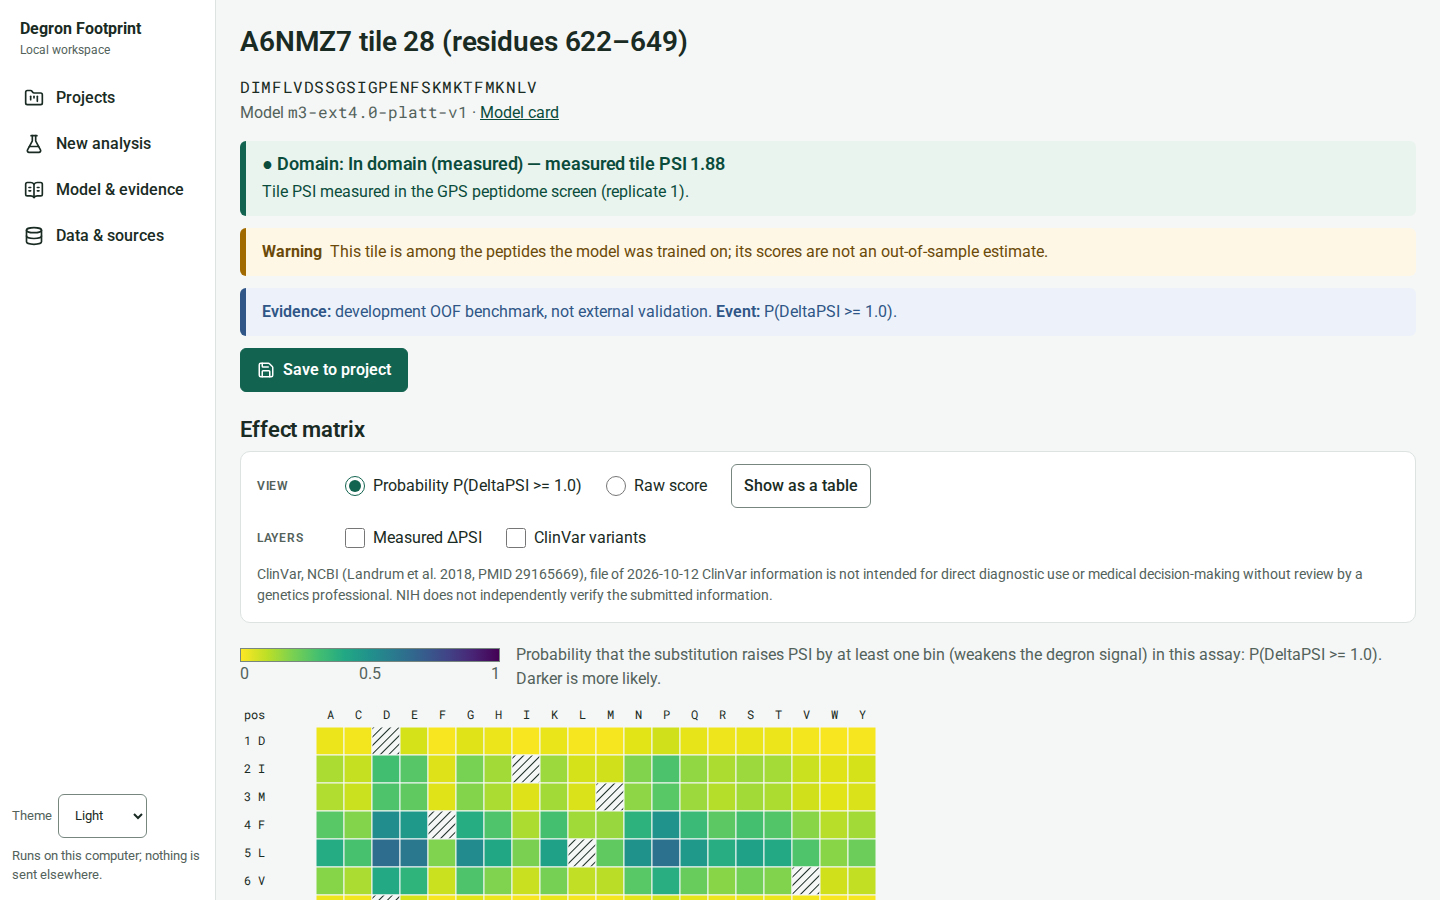
\includegraphics[width=0.92\textwidth]{assets/screenshots/05-result-matrix.png}
  \caption[The effect matrix as rendered by the application]{The effect matrix as rendered by the application. The domain banner and the warnings
  appear above the numbers by design. Wild-type cells are masked, and the legend states the event
  that the calibrated probability refers to. Captured from the running application with reference
  data, not from a mock-up.}
  \label{fig:app-matrix}
\end{figure}


\textbf{Tables and operations.} The ranking reads \texttt{analysis\_cell}; the shortlist and the
panel add no rows of their own and appear in the exported tables.

\textbf{Scientific constraint.} Ranking is meaningful only inside one tile. Batch and whole-protein
views therefore preserve tile identity and never present a single ordering across tiles, because no
evidence in the thesis supports cross-tile comparability. The priority panel also carries its
evidence label, ``retrospective, development benchmark'', ahead of the numbers in the document
order, so that a screen reader reaches the caveat before the figures.

\textbf{Evidence.} The interface unit tests assert both the ordering and the position of that label
relative to the numbers.

\subsection{Durable Batch and Whole-Protein Jobs}
\textbf{Purpose and user.} A researcher who wants to scan a complete protein, or a list of peptides,
cannot wait on a single request. This is UC-08, and it is where most of the engineering went.

\textbf{Flow.} The submission is previewed first: inputs are normalised, the number of windows is
reported together with coverage gaps and the configured limits, and the user confirms that the work
will be stored locally. A whole protein is tiled with a step of 23 residues, so window $n$ starts at
$(n-1)\cdot 23+1$ and spans 28 residues; only complete windows are generated and uncovered terminal
residues are reported rather than padded. Figure~\ref{fig:app-tiling} shows the rule on a real protein. The job pins the model, calibrator, gate and source
versions at submission. The worker then proceeds item by item as in
Figure~\ref{fig:app-job-sequence}, and the job state follows Figure~\ref{fig:app-job-states}.
Cancellation is accepted at any time and results already computed are kept.

\begin{figure}[htbp]
  \centering
  % Original schematic of whole-protein tiling (plan-report 5.4).
% Rule from the code (system/app/backend, whole-protein job; test_jobs.py
% test_whole_protein_windows_match_the_reference_tiles): window n starts at (n-1)*23+1 and spans
% 28 residues; only complete windows; uncovered terminal residues are reported, never padded.
% Example P60484 (PTEN, 403 residues): 17 windows cover 1-396, 397-403 uncovered, as on the job
% screen of the application. Deterministic arithmetic, no measured values.
\begin{tikzpicture}[fig, x=0.0325cm]
  % protein axis: 1 unit = one residue
  \draw[line width=1.2pt, oiGrey] (1,0) -- (403,0);
  \foreach \t in {1,100,200,300,403} { \draw (\t,-0.08) -- (\t,0.08); \node[dim, below] at (\t,-0.08) {\t}; }
  \node[font=\scriptsize, anchor=east] at (-4,0) {protein};
  % windows, alternating rows so that the 5-residue overlaps stay visible
  \foreach \n in {1,...,17} {
    \pgfmathtruncatemacro{\s}{(\n-1)*23+1}
    \pgfmathtruncatemacro{\e}{\s+27}
    \pgfmathsetmacro{\y}{mod(\n,2)==1 ? 0.45 : 0.8}
    \draw[draw=oiBlue, fill=oiSky!35] (\s,\y) rectangle (\e,\y+0.25);
  }
  \node[font=\scriptsize, anchor=east] at (-4,0.62) {windows};
  % uncovered tail
  \draw[draw=oiVermillion, pattern=north east lines, pattern color=oiVermillion] (397,0.45) rectangle (403,0.7);
  \draw[->, oiVermillion] (400,0.75) -- (400,1.25) node[above left=0pt and -6pt, font=\scriptsize, align=right] {397--403\\not covered};
  % zoom on two windows
  \draw[brace] (1,1.2) -- node[above=3pt, font=\scriptsize, anchor=south west, xshift=-14pt] {window 1: 1--28} (28,1.2);
  \draw[brace] (24,1.75) -- node[above=3pt, font=\scriptsize, anchor=south west, xshift=-14pt] {window 2: 24--51} (51,1.75);
  \node[note, text width=9.6cm, align=left, anchor=north west] at (1,-0.55)
       {Window $n$ starts at $(n-1)\cdot23+1$ and spans 28 residues, so neighbours share 5 residues.
        Example: PTEN (403 residues) gives 17 windows. Each window is scored in its own context;
        overlapping scores are never averaged and ranks stay within a window.};
\end{tikzpicture}

  \caption[Tiling of a whole protein into 28-residue windows]{Tiling of a whole protein into 28-residue windows with step 23. Windows are drawn in two
  rows only to show their 5-residue overlaps; terminal residues that do not fill a window are
  reported, not padded. Original schematic of the implemented rule.}
  \label{fig:app-tiling}
\end{figure}

\textbf{Tables and operations.} One path creates a job in a project and four read or control it:
submission, status, item listing, cancellation and export, all under \texttt{/v1/jobs}. They operate
on \texttt{analysis\_job} and \texttt{job\_item}.

\textbf{Scientific constraint.} A whole-protein scan is a collection of peptide-context predictions,
not a validated statement about the intact protein; overlapping windows keep their own context and
are never averaged into one number per residue.

\textbf{Evidence.} Figure~\ref{fig:app-job} shows progress with per-item outcomes. A protein of
\nAppProteinLen{} residues yields \nAppProteinTiles{} windows and completes in
\nAppProteinSeconds{}~s; one hundred peptides submitted together take \nAppPeptidesSeconds{}~s. The recovery requirement is tested by killing both processes while a job is in progress: after
a restart of \nAppRestartSeconds{}~s the job completes all \nAppProteinTiles{} windows with no
duplicated result.

\subsection{The Two-Tier Domain Gate}
\textbf{Purpose and user.} Any user can paste a sequence the model was never trained for. This
feature decides whether the system answers at all, and it is the place where a research result
directly governs software behaviour.

\textbf{Flow.} The gate from Section~\ref{sec:res-domain} is applied to every tile before scoring.
The first tier uses the screen stability of a known tile, the second predicts it from sequence when
no measurement exists, and both map their input through a fixed logistic function to a probability of
belonging to the training domain. Three states follow: inside, borderline, and outside. A tile
labelled outside is refused by default; the user may override it explicitly, and that override is
recorded with the result and travels into the export.

\textbf{Tables and operations.} The decision and its identifiers are stored on \texttt{tile} and on
each analysis, and the gate artefact is a \texttt{model\_version} row of its own, so a stored score
always names the gate that admitted it.

\textbf{Scientific constraint.} The intrinsic training threshold must not be compared with the
screen estimator directly; the earlier naive comparison was removed from the implementation, and the
frozen logistic rules are used instead. One consequence is deliberately visible to users: a minority
of the model's own training tiles are labelled outside the domain by the screen-based tier. That is a
property of the gate, which is accurate for the tiles it admits, and not a defect to be smoothed
away.

\textbf{Evidence.} Boundary fixtures cover the measured, predicted, borderline and override paths,
and golden tests tie the implemented logistic constants to the research script.

\subsection{Provenance, Export, and Imported Measurements}
\textbf{Purpose and user.} A result that cannot be traced is not usable in a thesis or a laboratory
notebook. This feature covers UC-03, UC-07 and UC-10, and it carries the narrower import and
comparison workflow of UC-05 and UC-09.

\textbf{Flow.} Saving is explicit and produces an immutable snapshot: inputs, model and calibrator
identity with hashes, gate decision, source versions, warnings and timestamps. Reopening reads that
snapshot; rerunning creates a new entry and never overwrites the old one. Export emits the analysis,
the job manifest including refused and failed items, or the comparison, as CSV or JSON with the same
provenance fields and the development-evidence label. Imports follow
Figure~\ref{fig:app-import-sequence}: staged, validated, explicitly committed, then available for
comparison against a saved analysis.

\begin{figure}[htbp]
  \centering
  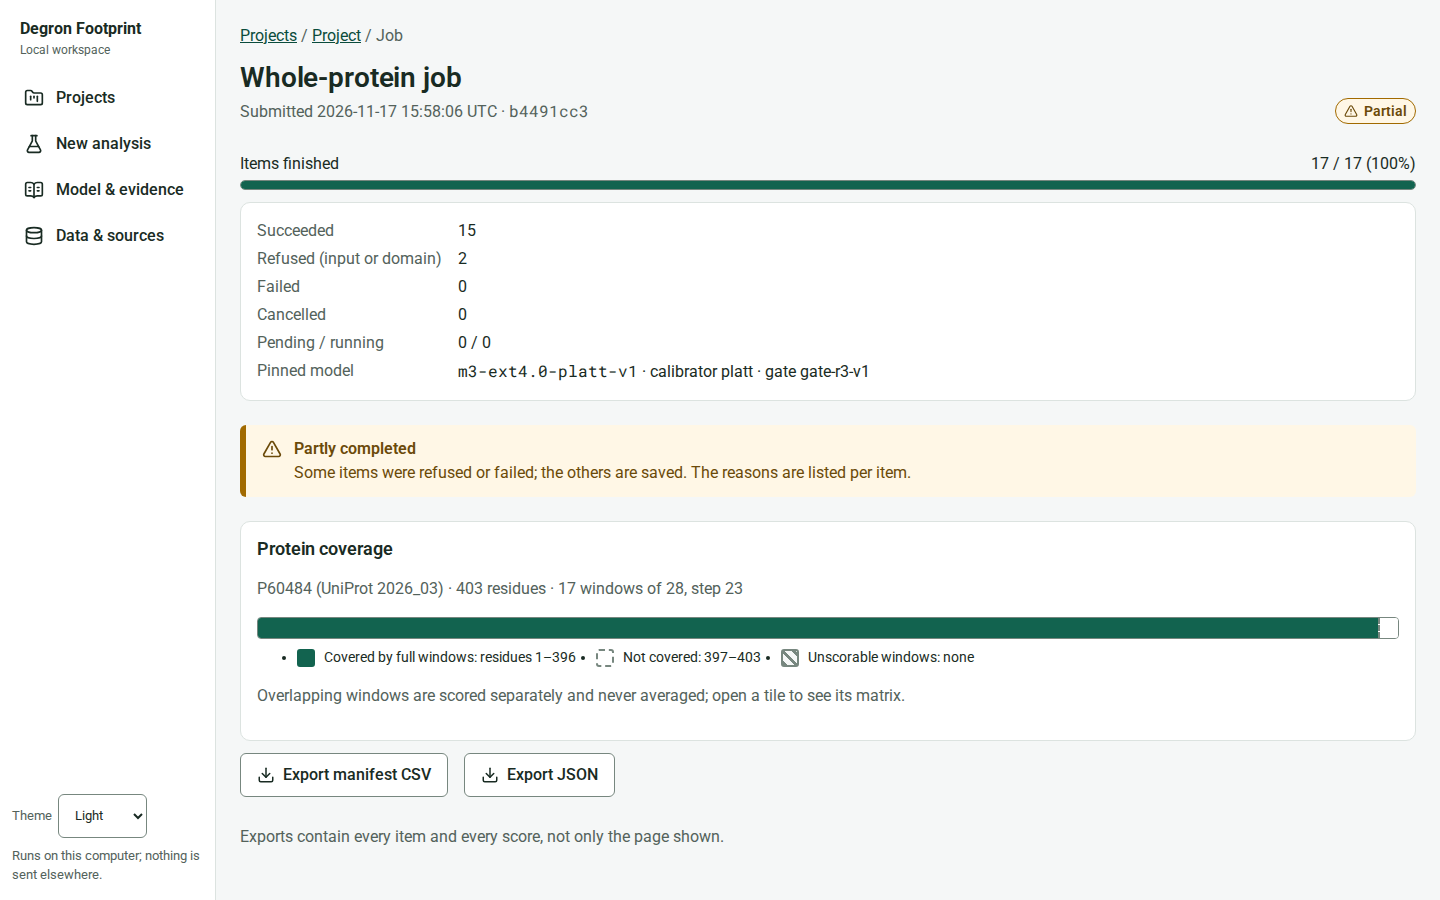
\includegraphics[width=0.92\textwidth]{assets/screenshots/06-job-progress.png}
  \caption[A durable job in progress]{A durable job in progress. Counts are shown per outcome, so a refused window is visibly
  distinct from a failure, and the job is reported as partial rather than successful when the gate
  refuses part of the protein.}
  \label{fig:app-job}
\end{figure}


\textbf{Tables and operations.} \texttt{GET} and \texttt{POST} on
\texttt{/v1/projects}, \texttt{/v1/analyses}, \texttt{/v1/datasets} and \texttt{/v1/comparisons},
with \texttt{/v1/models} and \texttt{/v1/sources} serving the evidence pages over
\texttt{model\_version} and \texttt{data\_source}.

\textbf{Scientific constraint.} Three rules are enforced rather than documented. An import never
retrains or modifies the model. Comparison metrics are computed only on rows whose endpoint and
units are comparable, with the number of such rows always reported, and incompatible endpoints are
shown side by side without a pooled metric. Missing values stay missing instead of becoming zero.
Finally, an imported measurement is not independent validation of the model, and the comparison
screen says so where the metrics appear.

\textbf{Evidence.} Figure~\ref{fig:app-model} shows the evidence page, which reads its content from
the model registry rather than from prose, and Figure~\ref{fig:app-comparison} shows a comparison
with its row counts. Export of a \nAppProteinTiles{}-window job manifest produces a \nAppExportMb{}~MB file in
\nAppExportSeconds{}~s, and a preview of \nAppImportRows{} imported rows completes in \nAppImportSeconds{}~s.

% FROZEN until plan-system G-SYS (plan-report 5.6): overall diagram/section, update once.
\section{Local Execution View}\label{sec:local-execution}
One computer hosts the browser, API, worker, database and workspace files. The release runs in two
equivalent ways. On the host, the API and the worker are started as two processes, or as one process
with the worker embedded. In containers, four long-running services come up together: the database,
the API, the worker and the web server, with a fifth one-off container that loads the reference data
from the research checkout read-only. A development profile adds hot reload. Only the web server
publishes a port, and only on the loopback address; the API, worker and database are reachable only
inside the container network. The same code supports PostgreSQL~16, the accepted local database,
and SQLite for isolated development and tests.

\begin{figure}[htbp]
  \centering
  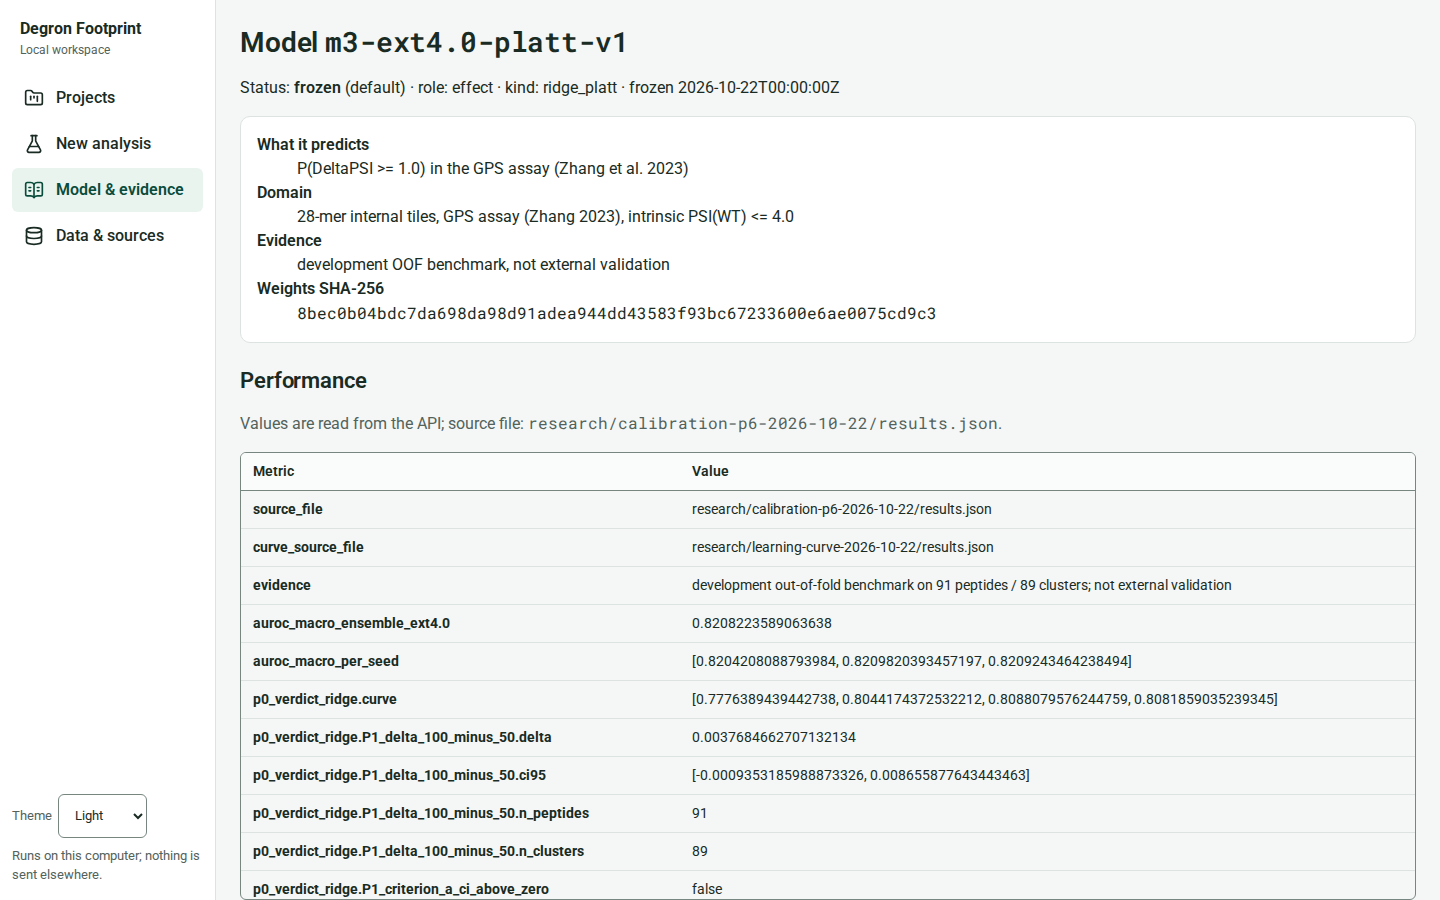
\includegraphics[width=0.86\textwidth]{assets/screenshots/12-model.png}
  \caption[The model and evidence page]{The model and evidence page. The served model, its calibrator, the domain gate and the
  reference sources are listed with their versions; the evidence boundary is stated on the page that
  users consult when they want to know what a score means.}
  \label{fig:app-model}
\end{figure}

\textbf{Two serving models.} The ridge model needs only numerical libraries; the adapted model needs
PyTorch and the protein language model, which are installed only when the container image is built
with that option, so the default image stays small. Switching between the models is a configuration
change and does not alter any stored analysis, because every snapshot names the model that produced
it. The adapted model reproduces the research implementation exactly, but it is slow on a processor
without acceleration: about \nAppLoraLatPfive{}~s per tile at the 95th percentile against
\nAppRidgeContainerPfive{}~ms for the ridge model in the same container, so it does not meet the proposed
300~ms target. The delivered configuration therefore keeps the ridge model as default. On the
author's own installation the adapted model has been set as default by configuration; that is a
local deployment choice, not a serving decision, and no decision record or supervisor approval
exists for it.

\begin{figure}[htbp]
  \centering
  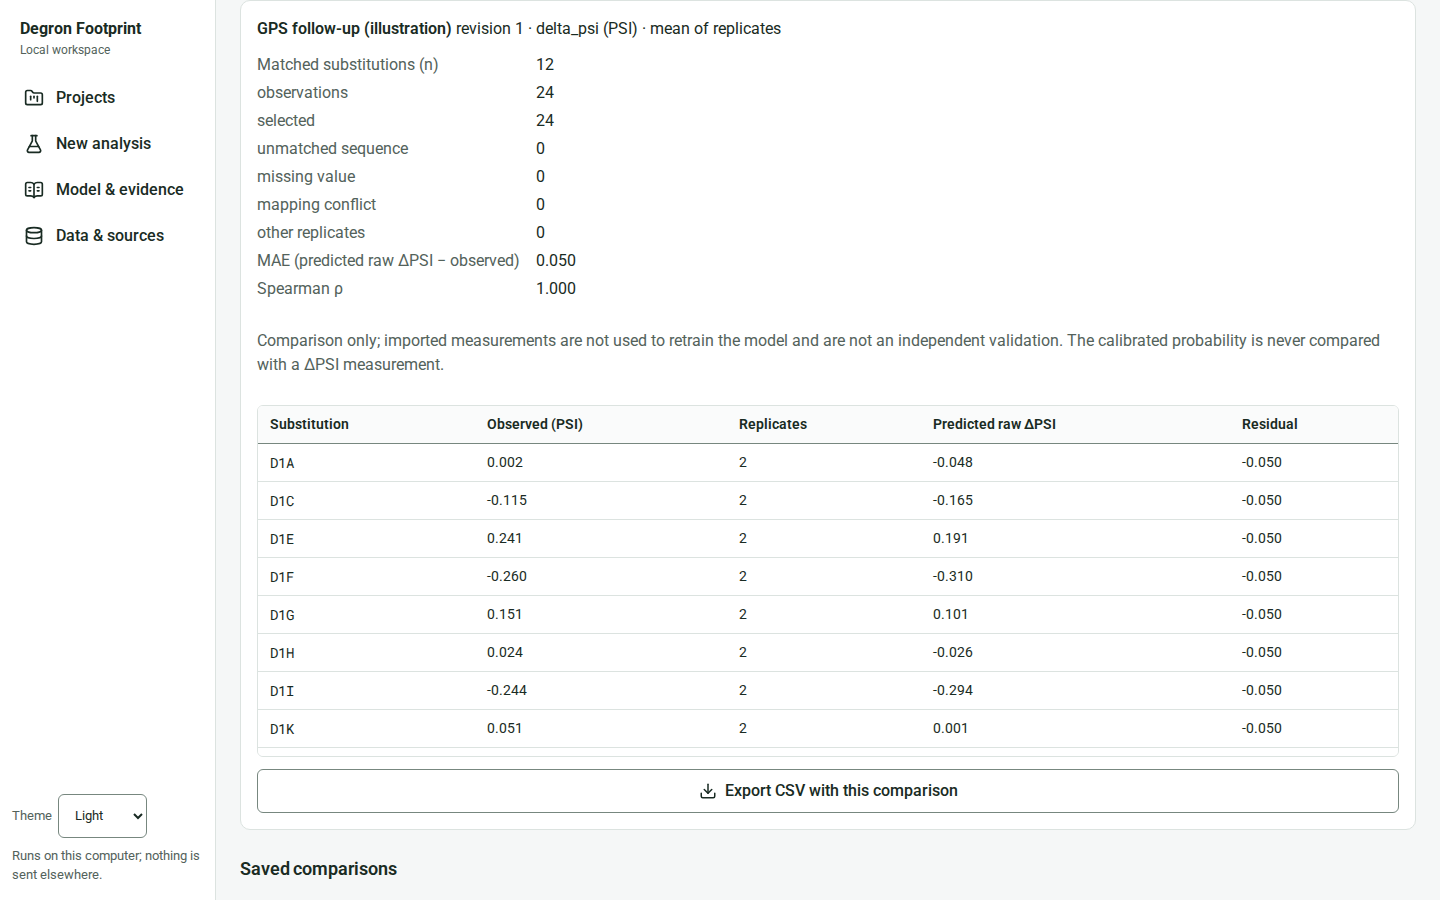
\includegraphics[width=0.86\textwidth]{assets/screenshots/08-comparison.png}
  \caption[Comparing predictions with imported measurements]{Comparing predictions with imported measurements. Matched, unmatched and conflicting row
  counts are shown with the metrics, and the imported dataset keeps its own assay metadata so that an
  incompatible endpoint cannot be pooled into a single score. The imported values in this
  illustration were derived from the prediction itself, so the near-perfect agreement shown is an
  artefact of the illustration and not a measurement.}
  \label{fig:app-comparison}
\end{figure}


\textbf{Security and privacy.} Cross-site write requests are refused, requests must declare a JSON
body, and the web server sends a strict content security policy with self-hosted fonts, so the page
loads nothing from another host. Biological sequences are never sent off the computer and never
appear in logs or URLs. The interface offers light and dark themes, adapts to widths from 360 to
1440~pixels, and uses fixed scientific colour scales: a reversed Viridis scale for probabilities and
PuOr for raw effects. Appendix~\ref{app:installation} gives the executed installation and startup
procedure for both the host installation and the container configuration.
